% %
% % Sample SBC book chapter
% %
% % This is a public-domain file.
% %
% % Charset: ISO8859-1 (latin-1) áéíóúç
% %
\documentclass{SBCbookchapter}
\usepackage[utf8]{inputenc}
\usepackage[T1]{fontenc}
\usepackage[brazil]{babel}
\usepackage{subfigure}
\usepackage{epsfig}
\usepackage{graphicx,url}
\usepackage{verbatim}
\usepackage{cite}
\usepackage{psfrag}
\usepackage{alltt}
\usepackage{indentfirst}
\usepackage{setspace}
\usepackage{amsmath}
\usepackage{amssymb}
\usepackage{listings}
\usepackage{color}
\usepackage{mathrsfs}
\usepackage{scalefnt}
\usepackage{colortbl}
\usepackage{float}
\usepackage{multirow}
\usepackage[table,xcdraw]{xcolor}
\newcolumntype{M}[1]{>{\centering\arraybackslash}m{#1}}


\definecolor{codegreen}{rgb}{0,0.6,0}
\definecolor{codegray}{rgb}{0.5,0.5,0.5}
\definecolor{codepurple}{rgb}{0.58,0,0.82}
\definecolor{backcolour}{rgb}{0.95,0.95,0.92}
 
\lstdefinestyle{codigo}{
    backgroundcolor=\color{backcolour},   
    commentstyle=\color{codegreen},
    keywordstyle=\color{codegreen},
    numberstyle=\tiny\color{codegray},
    stringstyle=\color{codepurple},
    basicstyle=\footnotesize,
    breakatwhitespace=false,         
    breaklines=true,                 
    captionpos=b,                    
    keepspaces=true,                 
    numbers=left,                    
    numbersep=5pt,                  
    showspaces=false,                
    showstringspaces=false,
    showtabs=false,                  
    tabsize=2
}
 
\lstset{style=codigo}

\setcounter{chapter}{2} 


\sloppy
\title{Processamento de Linguagem Natural para \\Identificação de Notícias Falsas em Redes Sociais:\\ Ferramentas, Tendências e Desafios\let\thefootnote\relax\footnote{Este capítulo foi realizado com recursos do CNPq, CAPES, RNP, FAPERJ, FAPESP (2018/23062-5) e Prefeitura de Niterói/FEC/UFF (Edital PDPA 2020).}
}



\author{Nicollas R. de Oliveira (UFF),
Pedro Silveira Pisa (Solvimm), \\Bernardo Costa (Solvimm), Martin Andreoni Lopez (Samsung Research), \\ Igor Monteiro Moraes (UFF), Diogo M. F. Mattos (UFF)
\vspace{-3mm}
}



\begin{document}
\maketitle

 
\begin{abstract}


The epidemic spread of fake news is a side effect of the expansion of social networks to circulate news, in contrast to traditional mass media such as newspapers, magazines, radio, and television. Human inefficiency to distinguish between true and false facts exposes fake news as a threat to logical truth, democracy, journalism, and credibility in government institutions. In this chapter, we present methods for preprocessing data in natural language, vectoring, dimensionality reduction, machine learning, and quality assessment of information retrieval. We also present a practical demonstration of identifying fake news will, from the collection and textual processing of social media news to the application of detection algorithms.

\end{abstract}

\begin{resumo}

A disseminação epidêmica de notícias falsas (\textit{fake news}) é um efeito colateral da expansão do uso de redes sociais como meio de circulação de notícias, em contraste às mídias tradicionais de comunicação massiva, como jornal, revista, rádio e televisão. A ineficiência humana para distinção entre fatos verídicos e falsos expõe as notícias falsas como uma ameaça à verdade lógica, à democracia, ao jornalismo e à credibilidade nas instituições de governo.
Este capítulo apresenta métodos de pré-processamento de dados em linguagem natural, vetorização, redução de dimensionalidade, aprendizado de máquina e avaliação da qualidade de recuperação de informação. Ao final do capítulo é apresentada uma demonstração prática do processo de identificação de notícias falsas, desde a coleta e processamento textual de notícias de mídias sociais até a aplicação algoritmos de classificação.
%O aumento da disseminação das notícias falsas (fake news) é resultado da expansão do uso de redes sociais que agilizam a propagação de boatos, sátiras e informações erradas. É difícil para um indivíduo diferenciar entre o que é verdadeiro e o que é falso enquanto é sobrecarregado com informações enganosas que são recebidas por repetidas vezes. Ademais, os indivíduos tendem a confiar em notícias falsas porque há atualmente uma descrença do público em relação às mídias tradicionais e, porque, muitas vezes tais notícias são compartilhadas por amigos ou confirmam um conhecimento prévio. Isso torna a identificação de notícias falsas mais crítica em comparação com outros tipos de informações, já que geralmente são apresentadas com elementos que lhe conferem autenticidade e objetividade, sendo relativamente mais fácil de obter a confiança do público. Por isso, a análise, a detecção e a intervenção em notícias falsas são desafiadoras. A análise estilístico-computacional baseada no processamento de linguagem natural é uma forma eficiente para identificar notícias falsas. O minicurso apresenta métodos de pré-processamento de dados em linguagem natural, vetorização, redução de dimensionalidade, aprendizado de máquina e avaliação da qualidade de recuperação de informação. Ao final do minicurso será apresentada uma demonstração prática do processo de identificação de notícias falsas, desde a coleta e processamento textual de notícias de mídias sociais, até a aplicação algoritmos de detecção. A demonstração será ambientada no Twitter em linguagem Python.
\end{resumo}

\section{Introdução}

A veracidade da informação é parte da essencial da sua integridade. O combate às notícias falsas torna indissociáveis os problemas de integridade e veracidade da informação em rede social e do consumo de dados na camada de aplicação. A divulgação de conteúdo falso implica desperdícios de recursos da rede e de processamento e, também, consiste em grave ameaça à integridade das informações e à credibilidade do serviço prestado~\cite{nicollasspl2020}. Dessa forma, o compartilhamento de informações inverídicas diz respeito à qualidade da confiança (\textit{Quality of Trust} - QoT) aplicada à distribuição de notícias~\cite{liu2010quality}, referindo-se a quanto um usuário confia em um conteúdo de uma determinada fonte. 

Em diferentes países, observam-se baixos níveis de confiança nas mídias de massa, \textit{e.g.} apenas 40\% nos Estados Unidos\footnote{Disponível em https://news.gallup.com/poll/185927/americans-trust-media-remains-historical-low.aspx.}, enquanto há altas porcentagens de compartilhamento de \textit{links} nunca lidos (\textit{blindshares}), \textit{e.g.} 59\% no Reino Unido \cite{gabielkov:hal-01281190}.
Em 2016, durante as eleições presidenciais dos Estados Unidos, a sociedade americana testemunhou uma epidemia alarmante de notícias falsas, cujos efeitos foram sentidos multilateralmente. Efeito semelhante foi sentido nas eleições de 2018 no Brasil. Devido ao seu potencial de disseminação, aceitação e destruição~\cite{science-spread-fakenews}, as notícias falsas são atualmente uma das grandes ameaças ao conceito de verdade lógica, deteriorando a democracia, o jornalismo, a justiça e até a economia~\cite{zhou2018fake,wang2017liar}. Esta última, em especial, teve de lidar com flutuações de 130 bilhões na bolsa de valores, como consequência de uma declaração falsa afirmando que Barack Obama havia se ferido em uma explosão\footnote{Disponível em https://www.forbes.com/sites/kenrapoza/2017/02/26/can-fake-news-impact-the-stock-market/\#559102f12fac.}. 
Nesse sentido, há um crescente esforço conjunto da comunidade acadêmica para desenvolver abordagens capazes de analisar, detectar e intervir na atuação desses conteúdos enganosos. Comprovações científicas já revelaram a vulnerabilidade dos humanos em distinguir verdade e falsidade, sendo reduzida a quase uma probabilidade aleatória, em média 54\% de acerto \cite{zhou2018fake,wang2017liar,rubin2010deception,rubin2016fake}.

O objetivo deste capítulo é apresentar os principais algoritmos e técnicas que auxiliam na caracterização linguística e detecção de notícias falsas em redes sociais para a garantia da integridade da informação. 
Este capítulo caracteriza o fenômeno~\cite{rubin2015deception,rubin2015towards}, investiga a propagação em mídias sociais e apresenta as ferramentas e os algoritmos para a detecção de notícias falsas.

O fator chave que impulsiona a criação de notícias falsas é que estas são criadas e publicadas {\it online}, de maneira mais rápida e barata quando comparadas a veículos tradicionais de mídia como jornais e televisão. Assim, o capítulo evidencia que embora a identificação de notícias falsas possa ser realizada manualmente por profissionais em jornalismo, o foco deste capitulo está na identificação automática através de aparato computacional. %A identificação de notícias falsas de maneira automática é o foco do capítulo. 
A identificação automática pode seguir abordagens distintas, como a prova automática de afirmações lógicas através de fatos já conhecidos, através da análise de propagação das notícias nas redes sociais, através da análise do perfil dos usuários que compartilham as notícias ou através do processamento de linguagem natural para a extração de conhecimento em uma abordagem estilístico-computacional~\cite{zhou2018fake}. O escopo do capítulo se limita à abordagem estilístico-computacional baseada em processamento de linguagem natural e justifica-se no fato de que o consumo de dados em redes sociais, por parte de usuários, está restrito à informação que chega ao usuário final. O usuário não tem acesso aos modelos de disseminação de conteúdo ou a modelos de reputação dos usuários que compartilharam os conteúdos consumidos. No capítulo são apresentas ainda as métricas de qualidade na extração das informações, assim como plataformas computacionais, disponíveis no mercado, que já executam o processamento de linguagem natural como serviço na nuvem. 

O restante do capítulo está organizado da seguinte forma. A Seção~\ref{sec:def} define o fenômeno da propagação de notícias falsas. Os métodos tradicionais de identificação de notícias falsas são discutidos na Seção~\ref{sec:metodos}. A criação de uma base de dados para identificação correta de notícias falsas é apresentada na Seção~\ref{sec:base}. A Seção~\ref{sec:nlp} descreve o processamento de dados em linguagem natural. A Seção~\ref{sec:vetorização} explica os processos para a transformação de textos em matrizes operáveis computacionalmente, enquanto a Seção~\ref{sec:aprendizado} apresenta as principais ferramentas de aprendizado de máquina usadas sobre dados em linguagem natural. A Seção~\ref{sec:solucoes-nuvem} elenca soluções comerciais em nuvens computacionais para tratamento de dados em linguagem natural e a Seção~\ref{sec:pesquisa} descreve iniciativas de pesquisas para a identificação de notícias falsas. Os desafios e oportunidades são discutidos na Seção~\ref{sec:desafios}. A Seção~\ref{sec:pratica} apresenta uma atividade prática para a identificação de notícias falsas. A Seção~\ref{sec:conclusao} realiza as considerações finais do trabalho.



\section{A Definição de Notícias Falsas}
\label{sec:def}

O termo notícias falsas (\textit{fake news}) originalmente faz referência a informações falsas e muitas vezes sensacionais divulgadas sob o disfarce de reportagem. Contudo, o uso desse termo evoluiu e, atualmente, é considerado sinônimo de propagação de informações falsas em mídias sociais~\cite{sharma2019combating}. Ressalta-se que, segundo o \textit{Google Trends}, o termo ``fake news'' alcançou grande popularidade entre os anos de 2017 e 2018, tendo o pico de popularidade em outubro de 2018, quando houve a eleição presidencial no Brasil~\footnote{Disponível em https://trends.google.com.br/trends/explore?date=all\&geo=BR\&q=fake\%20news.}. 

Notícias falsas são definidas como notícias que são intencionalmente e comprovadamente falsas~\cite{zhou2018fake}, ou, como quaisquer informações apresentadas como notícias que são factualmente incorretas e projetadas para enganar o consumidor, fazendo-o acreditar que são verdade~\cite{golbeck2018}. Sharma {\it et al.} argumentam que essas definições, no entanto, são restritas pelo tipo de informação ou pela intenção de engano e, portanto, não capturaram o escopo amplo do uso atual. Assim, Sharma {\it et al.} definem o termo como uma notícia ou mensagem publicada e propagada pela mídia, contendo informações falsas, independentemente dos meios e motivos por trás dela~\cite{sharma2019combating}. Apesar da inexistência de um consenso claro sobre o conceito de notícias falsas, a definição formal mais aceita interpreta como notícias intencionalmente e verificavelmente falsas. Com relação essa definição, destacam-se dois aspectos: a intenção e a autenticidade. O primeiro aspecto diz respeito à intenção desonesta usada com o intuito de enganar o leitor. Já o segundo se relaciona com a possibilidade de essas informações falsas terem sua veracidade verificadas.  

As notícias falsas podem ser diferenciadas pelos meios empregados para falsificar informações. O conteúdo das notícias pode ser completamente falso, totalmente fabricado para ludibriar o consumidor ou pode ser um conteúdo ardiloso que se utiliza de informações enganosas para abordar um determinado problema. Há também a possibilidade de serem usados conteúdos impostores que simulam fontes genuínas, mas, quando na verdade, as fontes são falsas. Outras características fraudulentas dos conteúdos de notícias falsas são também o uso de conteúdos manipulados, como manchetes e imagens que não estão de acordo com o conteúdo veiculado, ou também a contextualização da notícia com elementos falsos, assim como com conteúdo legítimo, porém em um contexto falso.

As notícias falsas também apresentam motivações ou intenções diversas. São identificadas como motivações para a criação e divulgação de notícias falsas as intenções de prejudicar ou desacreditar pessoas ou instituições; intenções de lucro para gerar ganhos financeiros aumentando a veiculação e a visualização de publicações \textit{online}; intenções de influenciar e manipular a opinião pública; assim como intenções de promover a discórdia ou, simplesmente, por diversão.

Diversos conceitos concorrem e se sobrepõem ao conceito de notícias falsas. Uma síntese desses múltiplos conceitos, não considerados notícias falsas, pode ser elencada como~\cite{rubin2015deception,shu2017fake,zhou2018fake,chen2015misleading}: 

\begin{enumerate}
    \item \textbf{sátiras e paródias}, que pelo conteúdo humorístico embutido, usando sarcasmos e ironias, é factível de ter seu caráter enganoso identificado; 
    \item \textbf{rumores e boatos}, que não se originaram de eventos de notícias, porém são aceitos publicamente; 
    \item  \textbf{teorias de conspiração}, por não serem facilmente verificáveis como verdadeiras ou falsas; 
    \item \textbf{\textit{spams}}, comumente associados a \textit{e-mails} não desejados, os \textit{spams} constituem  qualquer campanha publicitária que chega aos leitores por mídia sociais sem que sejam desejadas; 
    \item \textbf{trotes e embustes (\textit{hoaxes})} que são motivados apenas por diversão ou para enganar indivíduos direcionados; 
    \item \textbf{caça-cliques (\textit{clickbait})} que pelo fato de empregarem imagens em miniaturas, ou manchetes sensacionalistas, no processo convencimento de usuários a acessarem e compartilharem conteúdos duvidosos, mais se assemelham a um tipo de propaganda falsa;
    \item \textbf{desinformação (\textit{misinformation})} que é criada involuntariamente, sem uma origem ou intenção específica de desorientar o leitor; 
    \item \textbf{contra-informação (\textit{disinformation})} que são informações criadas com intenção específica de confundir o leitor.
\end{enumerate}

As características de cada um desses tipos de conteúdo fraudulento são comparadas às notícias falsas na Tabela~\ref{tab:comp}

%Apesar da inexistência de um consenso claro sobre o conceito de notícias falsas (\textit{fake news}), uma das definições formais mais aceitas as interpreta como notícias intencionalmente e verificavelmente falsas. Com relação a tal definição, destacam-se dois aspectos: a intenção e a autenticidade. O primeiro aspecto diz respeito à intenção desonesta usada com o intuito de enganar o leitor. Já o segundo se relaciona com a possibilidade de essas informações falsas terem sua veracidade checada. Uma vantagem dessa definição é a eliminação da ambiguidade gerada por diversos conceitos que frequentemente co-ocorrem e se sobrepõem ao conceito de notícias falsas. Uma síntese desses múltiplos conceitos, não considerados notícias falsas segundo essa definição, pode ser elencada como: (i) sátiras e paródias, que pelo conteúdo humorístico embutido, usando sarcasmos e ironias, é factível de ter seu caráter enganoso identificado; (ii) rumores e boatos, que não se originaram de eventos de notícias, porém são aceitos publicamente; (iii) teorias de conspiração, por não serem facilmente verificáveis como verdadeiras ou falsas; (iv) spam; (v) trotes e embustes (\textit{hoaxes}) que são motivados apenas por diversão ou para enganar indivíduos direcionados; (vi) caça-cliques (\textit{clickbait}) que pelo fato de empregarem imagens em miniaturas, ou manchetes sensacionalistas, no processo convencimento de usuários a acessarem e compartilharem conteúdos duvidosos, mais se assemelham a um tipo de propaganda falsa; (vii) \textit{misinformation} que é criada involuntariamente, sem uma origem ou intenção específica de desorientar o leitor; (viii) \textit{disinformation}~\cite{rubin2015deception,shu2017fake,zhou2018fake,chen2015misleading}. 

\begin{table}[h!]
\centering
\caption{Termos e conceitos relacionados à notícias falsas.}
\label{tab:comp}
\footnotesize
\begin{tabular}{|M{.27\textwidth}|M{.18\textwidth}|M{.22\textwidth}|M{.22\textwidth}|}
\cline{2-4}
\multicolumn{1}{c|}{} & \textbf{Autenticidade}  & \textbf{Intenção} & \textbf{Forma de Notícia}  \\ 
\hline 
Sátira e Paródias      & Falsa                  & Não Ruim          & Não               \\ 
\hline
Rumores e Boatos       & Desconhecida           & Desconhecida      & Desconhecido      \\ 
\hline
Teorias de Conspiração & Desconhecida           & Desconhecida      & Não               \\ 
\hline
Spam                   & Possivelmente Verdadeira   & Ruim / Publicitária & Não               \\ 
\hline
Trotes e Embustes      & Falsa        & Não Ruim          & Não               \\ 
\hline
Caça-cliques           & Possivelmente Verdadeira   & Publicitária      & Não               \\ 
\hline
Desinformação         & Falsa                  & Desconhecida      & Desconhecido      \\ 
\hline
Contra-informação         & Falsa                  & Ruim              & Desconhecido     \\
\hline
\end{tabular}
\end{table}

\subsection{As Características das Notícias Falsas}

O crescimento das comunicações mediadas por mídia social é um dos principais fatores que fomentam a mudança de características nas notícias falsas atuais~\cite{sharma2019combating}. A incapacidade de um indivíduo de discernir com precisão as notícias falsas das verdadeiras leva ao compartilhamento contínuo e à crença em informações falsas nas redes sociais~\cite{zhou2018fake,wang2017liar,rubin2010deception,rubin2016fake}. É difícil para um indivíduo diferenciar entre o que é verdadeiro e o que é falso enquanto é sobrecarregado com informações enganosas que são recebidas por repetidas vezes. Ademais, os indivíduos tendem a confiar em notícias falsas porque há atualmente uma descrença do público em relação às mídias tradicionais e, porque, muitas vezes tais notícias são compartilhadas por amigos ou confirmam um conhecimento prévio. Isso torna a identificação de notícias falsas mais crítica em comparação a outros tipos de informações, já que geralmente são apresentadas com elementos que lhe conferem autenticidade e objetividade, sendo relativamente mais fácil de obter a confiança do público.

A mídia social e o compartilhamento colaborativo de informações em plataformas \textit{online} fomentam também a propagação de notícias falsas, efeito chamado de câmara de eco (\textit{echo chamber effect})~\cite{shu2020fakenewsnet}.  O realismo ingênuo, em que os indivíduos tendem a acreditar mais facilmente nas informações que estão alinhadas a seus pontos de vista, o viés de confirmação, no qual os indivíduos procuram e preferem receber informações que confirmam seus pontos de vista existentes, e teoria da influência normativa, em que os indivíduos escolhem compartilhar e consumir opções socialmente seguras como uma preferência para aceitação e afirmação em um grupo social, são fatores importantes na percepção e compartilhamento de notícias falsas que fomentam o efeito da câmara de eco~\cite{shu2020fakenewsnet}. Esses conceitos implicam a necessidade de os indivíduos buscarem, consumirem e compartilharem informações que estejam alinhadas com suas visões e ideologias. Como consequência, os indivíduos tendem a formar conexões com indivíduos ideologicamente semelhantes e, de forma complementar, os algoritmos de recomendação de redes sociais tendem a personalizar recomendações de conteúdos que atendam às preferências de um indivíduo ou grupo. Esses comportamentos levam à formação de câmaras de eco e bolhas de filtro, em que os indivíduos ficam menos expostos a pontos de vista conflitantes e ficam isolados em sua própria bolha de informação~\cite{fuller2009, sharma2019combating}. O confinamento das notícias falsas em câmaras de eco ou bolhas de informação tendem a aumentar as suas sobrevida e divulgação, pois incorrem no fenômeno da credibilidade social, que sugere que a percepção das pessoas sobre a credibilidade de uma informação aumenta se os outros também a percebem como verdadeira, já que há a tendência de que indivíduos considerem como verídica uma informação a que são submetidos repetidas vezes~\cite{rubin2016fake}.

Os padrões de difusão de notícias falsas nas redes sociais têm sido frequentemente estudados para identificar as características das notícias falsas que auxiliam na discriminação entre notícias falsas e verdadeiras. O problema de identificação de notícias falsas pode ser definido de diversas formas. A classificação pode ser vista como a execução de uma classificação binária entre falsa ou verdadeira, boato ou não boato, farsa ou não farsa. Outra forma de definir o problema é como a execução de uma classificação de várias classes, verdadeira, quase verdadeira, parcialmente verdadeira, principalmente falsa ou falsa, ou ainda como rumor não verificado, rumor verdadeiro, rumor falso ou não é rumor~\cite{sharma2019fake}. A principal diferença entre a definição dos problemas de classificação é em função dos diferentes esquemas de anotação ou contextos de aplicativos em conjuntos de dados diferentes. Normalmente, os conjuntos de dados são coletados de declarações anotadas em sítios \textit{web} de verificação de fatos, como o ``Fato ou Fake"\footnote{Disponível em https://g1.globo.com/fato-ou-fake/.} ou a ``Agência Lupa"\footnote{Disponível em https://piaui.folha.uol.com.br/lupa/.}. Esses sítios refletem o esquema de rotulagem usado pela organização de verificação de fatos específica. 

Sharma {\it et al.} identificam três características relevantes para a identificação de notícias falsas: as fontes ou promotores da notícia; o conteúdo da informação; e a resposta do usuário ao receber a notícia em redes sociais~\cite{sharma2019combating}. A fonte ou os promotores da notícia têm grande influência na classificação da veracidade da notícia. Contudo, Sharma \textit{et al.} ressaltam que as listas de fontes possíveis de notícias falsas não são exaustivas e que os domínios usados para a divulgação de uma notícia podem ser falsificados~\cite{sharma2019combating}. Outro ponto a ser ressaltado é que {\it bots}, contas falsas ou comprometidas controladas por humanos ou programas para apresentar e promover informações nas redes sociais, são responsáveis por acelerar a velocidade de propagação de informações verdadeiras e falsas de forma quase igual, a fim de alavancar a credibilidade e a reputação das contas de \textit{bots}~\cite{botOrNot}. A segunda característica importante é o conteúdo da informação propagada. O conteúdo da informação é uma das principais características a ser analisada para classificar a notícia como verdadeira ou falsa. Oliveira {\it et al.} identificam que notícias falsas e notícias reais veiculadas no Brasil têm um comportamento estatisticamente diferente no somatório da frequência relativa das palavras usadas no conteúdo. Notícias falsas tendem a usar menos palavras relevantes do que notícias reais~\cite{nicollasspl2020}. Outras características textuais incluem o uso de palavras sociais, auto-referências, declarações de negação, reclamações e itens generalizantes, além de que há uma tendência de que notícias falsas apresentem menor complexidade cognitiva, menos palavras exclusivas, mais palavras de emoção negativa e mais palavras de ação~\cite{sharma2019combating}. Por fim, as respostas do usuário nas redes sociais fornecem informações auxiliares para a detecção de notícias falsas. A resposta dos usuários é importante para a identificação, pois, somada aos padrões de propagação, são mais difíceis de serem manipuladas do que o conteúdo da informação e, por vezes, as respostas dos usuários contêm informações óbvias sobre a veracidade~\cite{zhou2018fake}. O engajamento dos usuários, nas formas de curtidas, compartilhamentos, respostas ou comentários, contém informações capturadas na estrutura de árvores de propagação que indicam o caminho do fluxo de informações, informações temporais em carimbos de data e hora, informações textuais em comentários do usuário e informações de perfil do usuário envolvido no engajamento~\cite{sharma2019combating}.

A caracterização da fonte ou da propagação, do conteúdo e da reposta do usuário permitem definir diferentes técnicas de identificação de notícias falsas, tais como, identificação baseada em retroalimentação pelo padrão de propagação, identificação no processamento de linguagem natural aplicado ao conteúdo de mensagens e aplicação de mecanismos de aprendizado de máquina e, por fim, identificação baseada em intervenção dos usuários. Este capítulo foca nas soluções baseadas na análise do conteúdo das notícias.

\subsection{O Processo de Disseminação de Notícias Falsas}

Diversas entidades, indivíduos e organizações interagem na divulgação, moderação e consumo de notícias falsas nas redes sociais. Devido à pluralidade de atores envolvidos, o problema de identificação e mitigação da disseminação de notícias falsas torna-se ainda mais complexo. A divulgação das notícias falsas é fortemente baseada em mídias sociais em detrimento de mídias tradicionais de jornalismo, devido à grande escala, ao alcance das mídias sociais e à capacidade de compartilhar colaborativamente conteúdo. Os sítios \textit{web} de mídias sociais têm se tornado a forma mais popular de disseminação, devido à crescente facilidade de acesso e popularização da comunicação mediada por computador e do acesso à Internet~\cite{Mattos2019}. Paralelamente, enquanto nas mídias tradicionais de jornalismo a responsabilidade pela criação do conteúdo cabe ao jornalista e à organização redatora, a moderação nas redes sociais varia bastante. Cada mídia social está sujeita a diferentes regras de moderação e regulamentação de conteúdo. A informação é consumida principalmente pelo público em geral ou pela sociedade, que constituem número crescente de usuários de mídia social. O crescimento no consumo de informação por meio de mídia social aumenta o risco de notícias falsas causarem danos generalizados~\cite{sharma2019combating}.

Sharma {\it et al.} destacam três atores distintos na propagação das notícias falsas: o adversário, o verificador de fatos e o usuário susceptível~\cite{sharma2019combating}. Os adversários são indivíduos ou organizações mal-intencionados que muitas vezes se passam por usuários comuns de redes sociais usando {\it bots}~\cite{botOrNot} ou contas reais. Os adversários podem tanto agir como fonte ou como promotores de notícias falsas. Essas contas também agem em grupo propagando conjuntos de notícias falsas. O verificador de fatos consiste em um conjunto de várias organizações de verificação de fatos, como ``Fato ou Fake” e a ``Agência Lupa”,  que buscam expor ou confirmar notícias que gerem dúvidas sobre a sua veracidade. Muitas das vezes, as verificações se baseiam no jornalismo de checagem de fatos que depende da verificação humana. Contudo, há soluções tecnológicas automatizadas que visam a detecção de notícias falsas para empresas e consumidores. Essas soluções atribuem pontuações de credibilidade a conteúdo da {\it web} usando inteligência artificial. Por fim, o usuário susceptível consiste no usuário de rede social que recebe o conteúdo duvidoso, porém não é capaz de distinguir entre uma notícia falsa ou verídica e, assim, acaba propagando a notícia falsa em sua rede social, mesmo que não tenha a intenção de contribuir para a proliferação de conteúdo fraudulento.

\section{Os Métodos Tradicionais de Detecção de Notícias Falsas}
\label{sec:metodos}

A identificação de notícias falsas pode ser realizada por meios manuais, através de profissionais em jornalismo, sendo a abordagem mais utilizada normalmente. Contudo, tal abordagem não é compatível com o volume atual de criação e disseminação de conteúdo nas redes sociais. Para contrapor esse problema de escalabilidade, métodos automáticos geralmente integram técnicas de Recuperação de Informação, Processamento de Linguagem Natural (PLN) e Aprendizado de Máquina no processo de verificação da veracidade de notícias veiculadas na Internet. 

A respeito de métodos automáticos de detecção de notícias falsas, distinções podem ser observadas ao discretizar as formas de detecção por foco de atuação. Na literatura são vislumbradas três teorias analíticas preponderantes e potencialmente úteis na contenção de notícias falsas. A primeira teoria é fundamentada em uma \textbf{análise baseada na propagação}, cujo foco está no mapeamento qualitativo ou quantitativo do espalhamento das notícias falsas em rede sociais, a partir de padrões empíricos ou modelagem matemática, respectivamente. A base de ambos os mapeamentos é a cascata de notícias falsas, uma estrutura em árvore que representa todo o processo de disseminação de notícias falsas, podendo ser pautada tanto em uma perspectiva por saltos ou por tempo. A Figura \ref{fig:cascata} retrata as perspectivas de representação da propagação citadas.

\begin{figure}[tb!]
	\centering
	\includegraphics[width=1\columnwidth]{cascata_hop_time.png}
	\vspace{2mm}
	\caption{Ilustração das cascatas de notícias falsas, tanto numa perspectiva baseada em saltos (à esquerda) quanto baseada em tempo (à direita). O nó-raiz $A$, em ambas as perspectivas, representa o primeiro usuário a publicar ou criar a notícia falsa e os demais nós representam usuários atuantes no encaminhamento ou compartilhamento do conteúdo falso.}
	\label{fig:cascata}
    \vspace{-8mm}	
\end{figure}

Um desses padrões de propagação foi mapeado por Kwon \textit{et al.}, cujo estudo revelou uma tendência das notícias não-confirmadas exibirem múltiplos e periódicos picos de discussão ao longo do dia no \textit{Twitter}, enquanto que notícias confirmadas apresentavam apenas um pico proeminente \cite{kwon2013prominent}. Adicionalmente, os estudos de Zhou \textit{et al.} e Vosoughi \textit{et al.} alertaram sobre a capacidade das notícias falsas, sobretudo do âmbito político, se espalharem de maneira mais rápida, mais longe e com mais abrangência do que notícias verdadeiras. Tal conclusão foi embasada no comportamento da representação em cascata das notícias falsas, marcado por uma maior largura máxima, profundidade e tamanho, alcançados em menos tempo que a representação em cascata de notícias legítimas~\cite{zhou2015real,science-spread-fakenews}. 

Embora útil, a descoberta de padrões empíricos de propagação característicos de cada tipo de notícia é uma estratégia com resultados temporários, pois a alta dinamicidade e variabilidade de comportamento das notícias falsas. É conveniente a aplicação em conjunto com uma modelagem matemática. Em geral, essa modelagem recorre a uma análise regressiva usando modelos clássicos como o epidêmico e o econômico.

A construção matemática da difusão de notícias falsas através de uma modelagem epidêmica visa principalmente a predição do número de disseminadores (temperatura geral).
Essa estratégia de modelagem inicia com uma etapa que associa cada usuário a um dentre três estados: (i) disseminadores; (ii) potenciais disseminadores; e (iii) disseminadores arrependidos, aqueles que após encaminharem ou publicarem uma notícia falsa a apagam. Nesta etapa, há também a definição inicial das taxas de transição entre esses estados. A próxima etapa consiste na construção do modelo, a qual pode considerar fenômenos como o efeito \textit{backfire}~\footnote{Relacionado ao fato de indivíduos rejeitarem mais fortemente evidências opostas as suas crenças.} e o reflexo de Semmelweis~\footnote{Remete a tendência dos indivíduos rejeitarem novas evidências por estas contradizerem suas normas e crenças estabelecidas.}, que revelam a rejeição de indivíduos às ideias contrárias as suas. A terceira etapa consiste na determinação das taxas reais de transição entre estados~\cite{zhou2018fake}.

A modelagem econômica introduz uma abordagem racional sobre interações de notícias falsas, que tenta capturar e predizer o comportamento dos indivíduos ao serem expostos a uma notícia falsa. Neste tipo de modelagem, o ciclo de geração e consumo de notícias é visto como um jogo de estratégia entre dois jogadores, os publicadores e os consumidores.
A cada jogador, a decisão de encaminhar ou deletar uma notícia falsa implica pares de vantagens específicas e excludentes entre si. Aos publicadores, cabe a escolha entre obter uma vantagem de curto prazo ($g_{p}$), que maximiza o lucro relacionado ao número de consumidores alcançados, ou uma vantagem de longo prazo ($b_{p}$), que privilegia sua reputação, tornando-os uma fonte autêntica de notícias. Já para os consumidores, as consequências dessa decisão dual é dividida entre uma vantagem de informação ($g_{c}$), que permite a obtenção de informação verdadeira e não enviesada, ou uma vantagem psicológica ($b_{c}$), ligada à teoria de viés confirmatório que reflete sua preferência por receber notícias que satisfazem opiniões prévias e necessidades sociais. Dessa forma, quando $g_{p} > b_{p}$ e $g_{c} > b_{c}$ constrói-se uma cadeia propícia para o espalhamento de notícias falsas~\cite{shu2017fake}.

Paralelamente, existe a \textbf{análise baseada no usuário}, que considera o papel deste na disseminação das notícias, consequentemente distinguindo um usuário malicioso daqueles sem má intenção, os ingênuos. Sejam motivados por benefícios monetários ou não monetários, a atuação de usuários maliciosos nas redes sociais se dá através de contas que escondem a real identidade do gerenciador. Ao analisar o nível de participação de humanos no processo de gerenciamento dessas contas, pode-se dividi-las em trés categorias: \textit{social bots}, \textit{cyborgs} e \textit{trolls}. Todas essas contas maliciosas altamente ativas e partidárias têm um único propósito de tornarem-se fontes poderosas de proliferação de notícias falsas. Em um nível baixo de dependência humana, os \textit{social bots} são contas controladas por um algoritmo de computador, cujo objetivo é produzir conteúdo automaticamente e interagir com humanos ou outros \textit{bots}. Já em nível intermediário, os \textit{cyborgs} são contas que alternam entre atividades automatizadas e humanas. Normalmente, este tipo de conta maliciosa é registrado por um usuário humano, fornecendo assim uma camuflagem para definir programas automatizados para realizar atividades nas redes sociais. No nível mais elevado de dependência, os \textit{trolls} são contas totalmente mantidas por usuários humanos reais que visam perturbar comunidades \textit{online} e provocar uma resposta emocional dos consumidores~\cite{shu2017fake}.

%Em Shao (Shao et al., 2016), os autores expõem um método que descreve a extração de postagens que continham links para notícias falsas e páginas da web de checagem de fatos. Em seguida, eles analisaram a popularidade e os padrões de atividade dos usuários que publicaram esse tipo de postagem. Os autores concluíram que os usuários que propagam notícias falsas são muito mais ativos nas redes sociais do que os usuários que refutam as alegações (espalhando links de checagem de fatos). As descobertas dos autores também sugerem que há um pequeno conjunto de contas que geram grandes quantidades de notícias falsas em postagens. 
%De 14 milhões de mensagens espalhando 400 mil artigos no Twitter durante um período de dez meses em 2016 e 2017, Shao et al. encontrar evidências de que os bots espalharam notícias não confiáveis em um momento anterior em comparação com os humanos para aumentar as chances de um artigo se tornar "viral". (ver Fig. 18) [Shao et al. 2018]. Eles também descobrem que os humanos fazem a maioria das retuitar e retuitar artigos postados por [prováveis] bots quase tanto quanto os de outros humanos (ver Fig. 19)

Outros trabalhos, como Barreto {\it et al.}, propõem uma metodologia capaz de distinguir usuários legítimos e \textit{spammers} considerando a 2-vizinhança no \textit{Twitter}. A proposta é subdivida em três etapas, cuja primeira é a pré-seleção manual de possíveis usuários. Como critério de pré-seleção de um usuário malicioso utiliza-se o fato do usuário enviar mensagens contendo pelo menos um tópico popular. A segunda etapa inclui a coleta dos dados da rede no entorno dos usuários pré-selecionados. Como última etapa, é feita uma análise desses dados avaliando métricas como distribuição de grau, centralidade de grau, coeficiente de agrupamento e \textit{PageRank}. Ao final, os autores relatam um comportamento diferenciado da distribuição de grau dos \textit{spammers}, contrariando a lei de potência esperada para os usuários legítimos~\cite{barretospammers}.

Mesmo não intencionalmente, usuários comuns são igualmente susceptíveis a se tornarem propagadores de notícias falsas. Além da baixa capacidade de detecção de notícias falsas, usuários normais são influenciados por fatores psicológicos e sociais. Na psicologia, esses fatores são identificados como vulnerabilidades individuais cujo um dos exemplos conhecidos é o realismo ingênuo. Esta vulnerabilidade formula uma tendência dos usuários em acreditar que suas percepções da realidade são os únicos pontos de vista, enquanto as demais são consideradas desinformadas, irracionais ou tendenciosas. Considerando o campo social, a disseminação das notícias falsas está intimamente conectada à dinâmica social dos indivíduos, estando correlacionada à três teorias: (i) a Teoria da Prospecção, que descreve a tomada de decisão como um processo pelo qual os indivíduos fazem escolhas com base nos ganhos e perdas relativas em comparação com seu estado atual; (ii) a Teoria da Identidade Social, que associa o autoconceito dos indivíduos é derivado a partir da percepção de pertencimento a um grupo social relevante; (iii) a Teoria da Influência Normativa, na qual enfatiza que aceitação e afirmação social são essenciais para a identidade e autoestima de um indivíduo, fazendo com que os usuários escolham ser ``socialmente seguros''~\cite{shu2017fake}.

Embora a existência de notícias falsas preceda o surgimento das mídias sociais, seu advento alterou e ampliou a dinâmica de propagação desse tipo de informação, inclusive adicionando novos atores. Outro fator atual que facilita a disseminação desse tipo de notícia é o fenômeno de bolha social ou câmara de eco (\textit{echo chamber}) em que usuários tendem a se relacionar virtualmente com seus \textit{like-minders}, ou seja, pessoas que pensam como eles. Nessas bolhas sociais estão presentes duas ideias principais, sendo a primeira conhecida como credibilidade social. Tal ideia é explicada pelo fato de as pessoas serem mais propensas a considerar uma fonte como credível se os outros também a considerarem, especialmente quando não há como se comprovar. A segunda ideia remete a uma heurística de frequência, segundo a qual consumidores naturalmente preferem notícias que são ouvidas mais constantemente, mesmo sendo falsas \cite{shu2017fake}.

Uma terceira teoria analítica remete à \textbf{análise baseada no estilo} da escrita, cujo foco de atuação principal está no conteúdo da notícia, ou seja, no texto propriamente dito. Essa análise parte da premissa de que notícias falsas detêm perfis de escrita únicos, diferentes dos seus pares legítimos. Cabe então aos métodos de detecção alinhados com essa teoria aplicar técnicas para extração de características linguísticas.

Dentre os estudos relacionados a essa abordagem estilística, destaca-se o apresentado por Rashkin \textit{et al.}, que trabalha sob a hipótese de que as notícias falsas tendem a conter uma narrativa mais interessante a fim atrair leitores~\cite{rashkin2017truth}. Assim, utilizando um \textit{corpus} composto por artigos de notícias de diversas intenções, fontes e graus discretos de veracidade, o método empregado prevê a extração de características léxicas latentes. A análise dessas características permitiu formular perfis distintos de notícias dependendo da sua fonte de veiculação. Assim, constata-se que notícias oriundas de fontes confiáveis normalmente apresentam alguma forma de embasamento concreto, como comparações numéricas e expressões relativas a dinheiro. Em um sentido oposto, notícias de fontes menos confiáveis detinham uma incidência maior de pronomes de primeira e segunda pessoa, superlativos, advérbios de modo e palavras que expressam hesitação (\textit{hedging words}). A análise baseada no estilo é a explorada a seguir.%nas demais seções deste capítulo.

\section{A Construção da Base de Dados}
\label{sec:base}

A caracterização do problema de identificação de notícias como um problema de classificação implica a construção de uma base de dados adequada. A construção de uma base de dados com qualidade e disponibilidade é o pilar de qualquer mecanismo automático de detecção de notícias falsas. Sua importância está atrelada à necessidade de armazenar a máxima quantidade de exemplos contrastantes, notícias falsas e verdadeiras, para então serem absorvidos por algoritmos de aprendizagem de máquina~\cite{oshikawa2018survey}. A Tabela \ref{tab:datasets} traz uma compilação de bases de dados de notícias falsas disponíveis, tanto na língua inglesa quando em na língua portuguesa.

\begin{table} [tb!]
\label{tab:datasets}
\footnotesize
\centering
\caption{Base de dados de notícias falsas disponíveis}
\begin{tabular}{|M{.18\textwidth}|M{.14\textwidth}|M{.07\textwidth}|M{.3\textwidth}|M{.12\textwidth}|} 
\cline{2-5}
 \multicolumn{1}{c|}{} & \textbf{Conteúdo}             & \textbf{Quant.} & \textbf{Rotulagem}                                                                                                 & \textbf{Anotador}                               \\ 
\hline 
\textbf{Buzzface} \cite{santia2018buzzface}              & Postagens e comentários de redes sociais (Facebook) & 2263            & Granular em quatro níveis (predominantemente verdade, predominantemente falso, mistura de verdadeiro e falso e nenhum conteúdo factual) & Previamente checado por agências de notícias (Buzzfeed)                \\ 
\hline
\textbf{FAKENEWSNET} \cite{shu2020fakenewsnet}           & Artigos inteiros                                    & 23921           & Binária (verdadeiro ou falso)                                                                                                           & Previamente checado por agências de notícias (PolitiFact e GossipCop)  \\ 
\hline
\textbf{Fake.Br Corpus} \cite{monteiro2018contributions} & Artigos inteiros                                    & 7200            & Binária (verdadeiro ou falso)                                                                                                           & Considera a credibilidade da fonte                                     \\ 
\hline
\textbf{LIAR} \cite{wang2017liar}                        & Declarações curtas (políticas)                      & 12,8k           & Granular em seis níveis (verdade, predominantemente verdade, meia-verdade, quase verdade, falso, \textit{pants-fire})                            & Previamente checado por agências de notícias (PolitiFact)              \\ 
\hline
\textbf{Emergent} \cite{ferreira2016emergent}            & Declarações e títulos relacionados                  & 300             & Binária (verdadeiro ou falso)                                                                                                           & Equipe jornalística                                                    \\ 
\hline
\textbf{FEVER} \cite{thorne-etal-2018-fever}             & Declarações curtas (Wikipedia)                      & 185k            & Granular em três níveis (suportada, refutada e sem informação suficiente)                                                               & Anotadores humanos treinados                                           \\ 
\hline
\textbf{CREDBANK} \cite{mitra2015credbank}               & Postagens de redes sociais (Twitter)                & 60M             & Vetor com 30 dimensões contendo pontuações variáveis em cinco níveis de veracidade                                                      & Crowd-sourcing                                                         \\ 
\hline
\textbf{BuzzfeedNews}                                                   & Postagens de redes sociais (Facebook)               & 2282            & Granular em quatro níveis                                                                                                               & Equipe jornalística                                                    \\ 
\hline
\textbf{BuzzFeed-Webis} \cite{potthast2017stylometric}   & Postagens de redes sociais (Facebook)               & 1687            & Granular em quatro níveis                                                                                                               & Previamente checado por agências de notícias (Buzzfeed)                \\ 
\hline
\textbf{PHEME} \cite{zubiaga2016analysing}               & Postagens de redes sociais (Twitter)                & 330             & Binária (verdadeiro ou falso)                                                                                                           & Jornalistas e crowd-sourcing                                           \\
\hline
\end{tabular}
\vspace{-8mm}
\end{table}

Nesse contexto, uma eventual coleta errônea de dados tem o potencial de causar inúmeras consequências negativas, que variam desde a particularização da análise até a obtenção de resultados dissonantes. Logo, é prudente adotar algumas diretrizes sugeridas por Rubin \textit{et al.} para a formação de um \textit{corpus} de notícias falsas~\cite{rubin2015deception}. Rubin {\it et al.} defendem que qualquer construção de uma base de dados, \textit{corpus}, de notícias falsas deve se ater a nove condições importantes, elencadas a seguir. (i) Considerar tanto as instâncias falsas como as verdadeiras permite que eventuais métodos preditivos aplicados à base considerem padrões característicos de cada tipo de notícia. (ii) A informação deve estar preferencialmente em formato textual, em vez de ser apresentada como mídia em formato de áudio ou vídeo. Informações nesses formatos devem ser transcritas, tornando-se manipuláveis por ferramentas de processamento de linguagem natural. (iii) A homogeneidade das notícias quanto ao tamanho e (iv) quanto a maneira da escrita, são outras duas condições a serem consideradas, evitando sempre que possíveis instâncias muito díspares. Igualmente, existe uma preocupação com (v) a forma de distribuição das notícias, visto que há suspeitas de que ao saber como e em qual contexto estas foram fornecidas, \textit{e.g.} humorístico, sensacionalista, pode-se influenciar os leitores. Além disso, (vi) a aquisição de notícias de um mesmo intervalo temporal é um fator primordial, pois os assuntos podem variar drasticamente em um curto intervalo de tempo. Adicionalmente, (vii) é aconselhável atender alguns aspectos pragmáticos, tais como custos com direito autoral, disponibilidade, facilidade de obtenção e privacidade dos escritores. Não se deve negligenciar o (viii) idioma e a (ix) cultura a que pertencem os dados coletados, pois a tradução pode implicar ambiguidades ou más interpretações, afetando negativamente a eficiência de processos de detecção~\cite{rubin2015deception,rubin2014pragmatic}.

%%%%%%%%%%

\section{Processamento de Linguagem Natural}
\label{sec:nlp}

O Processamento de Linguagem Natural (PLN), também conhecido como linguística computacional, consolida-se como um campo de pesquisa que envolve modelos e processos computacionais para a solução de problemas práticos de compreensão e manipulação de linguagens humanas. Independentemente de sua forma de manifestação, textual ou fala, a linguagem natural é entendida como qualquer forma de comunicação diária entre humanos. Tal definição exclui linguagens de programação e notações matemáticas, consideradas linguagens artificiais. As linguagens naturais estão em constante mudança, dificultando o estabelecimento de regras explícitas para computadores~\cite{clark2012automatically, otter2020survey, bird2009natural}.

\begin{figure}[tb!]
	\centering
	\includegraphics[width=1\columnwidth]{nlp_schema_layers.png}
	\vspace{4mm}
	\caption{Aplicação do processamento de linguagem natural em um texto bruto. A tokenização segmenta o texto contíguo em um conjunto de \textit{tokens}. Elementos de pouca relevância semântica são removidos, assim como pontuações, caracteres especiais e \textit{stopwords}. Entidades nomeadas são identificadas e removidos. \textit{Stemização} ou \textit{lematização} reduzem a diversidade de \textit{tokens}.}
	\label{fig:esquema_nlp}
	\vspace{-8mm}
\end{figure}

\begin{table}[tb!]
\caption{Características usadas em cada abordagem de detecção de notícias falsas baseadas em processamento de linguagem natural.}
\centering
\footnotesize
\begin{tabular}{|M{2cm}|l|l|l|l|l|l|l|l|} 
\cline{3-9}
\multicolumn{1}{l}{}           &                                          & \rotatebox[origin=c]{90}{ \cite{zhou2004automating} }                   & \rotatebox[origin=c]{90}{ \cite{fuller2009} }                 & \rotatebox[origin=c]{90}{ \cite{afroz2012detecting} }                & \rotatebox[origin=c]{90}{\cite{hauch2015computers}}               & \rotatebox[origin=c]{90}{ \cite{monteiro2018contributions} }              & \rotatebox[origin=c]{90}{ \cite{rashkin2017truth} }              & \rotatebox[origin=c]{90}{ \cite{rubin2016fake} }                 \\ 
\hline
\textbf{\textbf{Tipo}}      & \multicolumn{1}{c|}{\textbf{\textbf{Atributos}} } &                       &                         &                        &                        &                           &                          &                         \\ 
\hline
\multirow{9}{*}{Quantidade}    & Contagem de caracteres ou \textit{tokens}                                                         & x                     &                         & x                      &                        & x                         &                          &                         \\ 
\cline{2-9}
                               & Contagem de palavras                                                                     &                       & ~x                      & x                      & x                      & x                         &                          &                         \\ 
\cline{2-9}
                               & Contagem de sentenças                                                                    & x                     & x                       & x                      & x                      & x                         &                          &                         \\ 
\cline{2-9}
                               & Contagem de verbos                                                                       & x                     & x                       &                        & x                      &                           & x                        &                         \\ 
\cline{2-9}
                               & Contagem de frases nominais$^1$                                                           & x                     &                         &                        &                        &                           &                          &                         \\ 
\cline{2-9}
                               & Contagem de substantivos                                                                 &                       &                         &                        &                        & x                         &                          &                         \\ 
\cline{2-9}
                               & Contagem de \textit{stopwords}                                                                    &                       &                         &                        &                        & x                         &                          & x                       \\ 
\cline{2-9}
                               & Contagem de adjetivos                                                                    &                       &                         &                        &                        & x                         &                          & x                       \\ 
\cline{2-9}
                               & Contagem de modificadores$^2$                                                                & x                     & x                       & x                      &                        & x                         & x                        & x                       \\ 
\hline
Informalidade                  & Taxa de erros tipográficos                                                               & x                     &                         &                        & x                      & x                         &                          &                         \\ 
\hline
\multirow{4}{*}{Complexidade}  & Média de caracteres por palavra                                                          & x                     & x                       & x                      & x                      &                           &                          &                         \\ 
\cline{2-9}
                               & Média de palavras por sentença                                                           & x                     & x                       & x                      & x                      & x                         &                          &                         \\ 
\cline{2-9}
                               & Média de orações por sentença                                                            & x                     &                         &                        &                        &                           &                          &                         \\ 
\cline{2-9}
                               & Média de pontuações por sentença                                                         & x                     & x                       & x                      &                        & x                         &                          &                         \\ 
\hline
\multirow{6}{*}{Incerteza}     & \% de verbos modais                                                                      & x                     & x                       & x                      & x                      & x                         & x                        &                         \\ 
\cline{2-9}
                               & \% de termos que indicam certeza$^3$                                                         & x                     & x                       & x                      & x                      &                           & x                        &                         \\ 
\cline{2-9}
                               & \% termos que indicam generalização                                                      &                       & x                       &                        & x                      &                           & x                        &                         \\ 
\cline{2-9}
                               & \% termos que indicam tendência                                                          &                       & x                       & x                      & x                      &                           &                          &                         \\ 
\cline{2-9}
                               & \% de números e quantificadores$^4$                                                         &                       &                         & x                      & x                      &                           & x                        &                         \\ 
\cline{2-9}
                               & \# de pontos de interrogação                                                             &                       &                         & x                      &                        &                           &                          &                         \\ 
\hline
\multirow{4}{*}{Não Imediação} & \% de voz passiva                                                                        & x                     & x                       &                        & x                      & x                         &                          &                         \\ 
\cline{2-9}
                               & Pronomes na 1$^a$ pessoa do singular                                                         & x                     & x                       & x                      & x                      & x                         & x                        & x                       \\ 
\cline{2-9}
                               & Pronomes na 1$^a$ pessoa do plural                                                           & x                     & x                       & x                      & x                      & x                         & x                        & x                       \\ 
\cline{2-9}
                               & Pronomes na 2$^a$ ou  3$^a$ pessoa do plural                                                      & x                     & x                       & x                      & x                      & x                         &                          & x                       \\ 
\hline
\multirow{4}{*}{Diversidade}   & Diversidade Léxica: \% palavras únicas                                                   & x                     & x                       & x                      & x                      &                           &                          &                         \\ 
\cline{2-9}
                               & Redundância: \% de \textit{function words}$^5$                                                        & x                     & x                       & x                      & x                      &                           &                          &                         \\ 
\cline{2-9}
                               & \% de \textit{content words}$^6$                                                                      & x                     & x                       &                        & x                      &                           &                          &                         \\ 
\cline{2-9}
                               & Entidades nomeadas aleatórias$^7$                                                            &                       &                         &                        &                        &                           &                          & x                       \\ 
\hline
\multirow{4}{*}{Sentimento}    & \% de palavras positivas                                                                 & x                     & x                       & x                      & x                      & x                         &                          &                         \\ 
\cline{2-9}
                               & \% de palavras negativas                                                                 & x                     & x                       & x                      & x                      & x                         &                          & x                       \\ 
\cline{2-9}
                               & \# de pontos de exclamação                                                               &                       &                         & x                      &                        &                           &                          &                         \\ 
\cline{2-9}
                               & Teor humorístico/sarcástico                                                              &                       &                         &                        &                        &                           &                          & x                       \\
\hline
\end{tabular}\\
\footnotesize{$^1$frases cujos núcleos são substantivos. $^2$adjetivos e advérbios. $^3$e.g. ``nunca'', ``sempre''. $^4$advérbios de intensidade. $^5$palavras com pouco significado atrelado, usadas para expressar relações gramaticais entre palavras ou especificar a atitude ou o humor do falante, e.g., preposições, pronomes, verbos auxiliares, conjunções e artigos. $^6$palavras que contém um conteúdo semântico, e.g., substantivos, verbos, adjetivos e a maioria dos advérbios. $^7$presença de nomes próprios, nunca antes citados no texto, na última sentença.}\\
\vspace{-5mm}
\label{tab:caracteristicas}
\end{table}

Em uma decomposição refinada, o PLN pode ser dividido em cinco estágios primários de análise, que, quando realizados, permitem que o significado pretendido pelo autor seja extraído computacionalmente de um documento textual. Embora seja mais condizente com um estágio de pré-processamento, o primeiro estágio é a segmentação por \textit{tokenização}. A \textit{tokenização} é uma técnica obrigatória dado que os documentos textuais em linguagem natural geralmente são compostos de frases longas, complicadas e mal formadas. A etapa seguinte é a análise léxica, que visa relacionar as variantes morfológicas aos seus \textit{lemas}, ou seja, a forma primitiva das palavras do dicionário. A análise sintática foca no relacionamento das palavras entre si, cada uma assumindo seu papel estrutural nas frases, e de como as frases podem ser partes de outras, constituindo sentenças. Linguisticamente, a análise semântica tenta destilar o significado de palavras, expressões fixas, sentenças inteiras, sendo assim frequentemente aplicada na resolução de ambiguidades. Por fim, a análise pragmática busca compreender uma determinada frase, observando referências pronominais % ou pronominais 
e a coerência textual da estrutura das frases adjacentes. Embora o PLN possa introduzir outros estágios de análise, como reconhecimento de emoção, esses cinco estágios básicos são suficientes para extrair a informação semântica contextualizada de um documento de linguagem natural~\cite{dale2010}.

Limitando o processamento até o estágio de análise morfológica, é possível compor uma sequência básica de técnicas de PLN para garantir a identificação, e posterior remoção, de qualquer ruído textual que possa comprometer a extração e interpretação inteligente das informações contidas em cada sentença.
Nesta sequência, ilustrada na Figura~\ref{fig:esquema_nlp}, são aplicadas técnicas de limpeza e conformação dos dados incluindo
\textit{tokenização}, remoção de pontuação e caracteres especiais, eliminação de \textit{stopwords}, correção ortográfica, reconhecimento de entidades nomeadas e \textit{stemização} ou \textit{lematização}. Guiada pela ordem acima mencionada, cada \textit{sentença} do texto original é primeiramente submetida a um procedimento de discretização visto na Etapa 1, conhecido como \textit{tokenização}. Usando neste caso o caractere de espaço como critério delimitador, a \textit{tokenização} transforma cada sentença contígua em uma lista de \textit{tokens}, permitindo o manuseio individualizado dos \textit{tokens}. Basicamente cada \textit{token} é visto como uma instância de uma sequência de caracteres. Posteriormente na Etapa 2, recursos ortográficos como pontuação, \textit{e.g.} pontos final, de exclamação e de interrogação, e caracteres especiais, \textit{e.g.} números, cifrão e asterisco, são removidos de cada \textit{token}.

Na Etapa 3, eliminam-se as \textit{stopwords}, ou palavras mais frequentes, como conectivos, artigos e pronomes. Essa tarefa em especial tem como base o princípio de que quanto maior a frequência de uma palavra no \textit{corpus}, menos informação relevante a palavra possui. Em seguida na Etapa 4, ocorre a correção ortográfica através da comparação do \textit{token} com seu correspondente mais próximo no dicionário. Executa-se tal procedimento calculando a distância Levenshtein, \textit{i.e.}, o número mínimo de operações necessárias para transformar um nome no banco de dados em outro contido em um dicionário de nomes. O reconhecimento de entidades nomeadas, Etapa 5, identifica principalmente nomes próprios, com subsequente remoção dessas palavras. Por fim, com o objetivo de reduzir o processamento desnecessário causado por eventuais redundâncias entre as palavras, seja por flexões ou derivações, é comum a adoção da Etapa 6a ou 6b, sendo respetivamente a \textit{lematização} e a \textit{stemização}. Na tarefa de \textit{lematização}, procura-se eliminar as possíveis variantes ou plurais de uma mesma palavra, reduzindo-as ao mesmo lemas, conhecidos como forma de dicionário. Em contrapartida, na \textit{stemização} esta redução é feita transformando cada palavra no seu radical~\cite{icnc-2020-nicollas, navigli2009word,manning1999foundations}.
 
Expandindo o processamento textual a outros estágios linguísticos, há técnicas de PLN que desempenham a tarefa de análise sintática em diferentes graus de complexidade. Em um nível básico, a POS (\textit{part-of-speech}) \textit{tagging} caracteriza-se como uma técnica que retorna apenas a camada mais inferior da árvore de análise, ou seja, a marcação gramatical. Assim, a cada palavra de sentença é atribuído um meta-dado, identificando sua classe gramatical e conjugação. Em um nível intermediário, a técnica \textit{chunking}, também chamada de análise superficial, é uma técnica que analisa frases inteiras, primeiro identificando as partes constituintes das frases (substantivos, verbos, adjetivos) e, em seguida, ligando-as a unidades de ordem superior com significado gramatical discreto. Através dessa técnica, é selecionar estruturas sintáticas específicas como frases nominais, verbais~\cite{manning2014stanford}.

%Seria legal colocar como essas técnicas de PLN são implementadas computacionalmente

A análise de sentimento, ou mineração de opinião, inspeciona o texto fornecido e identifica a atitude ou emoção dominante no texto através de um grau de polaridade, classificando-o como positivo, negativo ou neutro. Outra propriedade comumente associada à análise de sentimento é a subjetividade, que permite diferenciar frases com alta incidência de opinião, julgamento ou emoção das frases com informações factuais. Normalmente a classificação do sentimento de frases funciona considerando as palavras isoladamente, atribuindo pontos positivos para palavras positivas e pontos negativos para palavras negativas e, em seguida, resumindo esses pontos. A simplicidade dessa lógica resulta em um desprezo pela ordem das palavras implicando perdas semânticas relevantes\cite{socher2013recursive}.
Modelos online atuais consideram a estrutura da sentença e constro\~em a representação de sentenças inteiras. Assim, esses modelos calculam o sentimento baseados em como as palavras da sentença compõem o significado de frases longas. 

Atualmente, dentre as ferramentas mais poderosas de extração de conhecimento sobre textos, a Stanford CoreNLP~ \footnote{Disponível em https://stanfordnlp.github.io/CoreNLP/.} e a NLTK~\footnote{Disponível em https://www.nltk.org/.} são as mais conhecidas.
Outras ferramentas como a Consulta Linguística e Contagem de Palavras, \textit{Linguistic Inquiry and Word Count} - LIWC)~\cite{pennebaker2001linguistic} destaca-se como um software de análise textual capaz de analisar e quantificar os componentes emocionais, cognitivos e estruturais presentes nos textos. A capacidade do LIWC revelar características latentes de um texto é intimamente dependente do idioma do dicionário de palavras associado ao software. Embora originalmente otimizado para a língua inglesa, atualmente o dicionário LIWC foi traduzido para a língua portuguesa\cite{balage2013evaluation}. Essas ferramentas são igualmente úteis na extração de características como as vistas na Tabela \ref{tab:caracteristicas}. 

%reescrevi só pq não sei se foi copiado de alguma parte...
%Contudo, atualmente há modelos \textit{online} que constroẽm uma representação de sentenças inteiras com base na estrutura da sentença. Ele calcula o sentimento com base em como as palavras compõem o significado de frases mais longas.
%alternativa a essa lógica é modelo 
%Diante das possibilidade, os análise de sentimento é especialmente útil na identificação de discursos de ódio


\section {Representação Vetorial de Textos}
\label{sec:vetorização}

Mesmo devidamente padronizada, cada sentença não é passível de ser operada matematicamente, visto que ainda é composta por radicais de palavras e não por valores mensuráveis. Destaca-se que até este momento, as operações realizadas sobre os dados são realizadas em cadeias de caracteres. No entanto, para o cálculo de modelos de aprendizado de máquina são necessários dados que possam ser operados matematicamente. Para obter uma representação numérica, emprega-se o Modelo de Espaço Vetorial. Esse modelo define que textos, sejam sentenças ou documentos, podem ser interpretados como um espaço vetorial de palavras, em que cada palavra pode ser representada em diferentes padrões, tais como: o binário, Saco-de-Palavras, Frequência do Termo -- Inverso da Frequência nos Documentos (\textit{Term Frequency–Inverse Document Frequency}, TF-IDF). Para ilustrar as particularidades de cada padrão de vetorização, considera-se o \textit{corpus}~\footnote{Linguisticamente, um \textit{corpus} é uma coletânea de documentos sobre determinado tema. Um conjunto de \textit{corpus} é denominado \textit{corpora}.} da Tabela~\ref{tab:corpus} formado por uma coletânea de quatro documentos, cada um contendo apenas uma única sentença.
Devido à unicidade na quantidade de sentenças adotada no \textit{corpus} exemplo, as descrições a seguir mostram as possíveis representações vetoriais em nível de documento e não em nível de sentença, embora isto seja igualmente viável.

\begin{table}[h]
\centering
\caption{\textit{Corpus} exemplo}
\begin{tabular}{
>{\columncolor[HTML]{EFEFEF}}c cllllllllll}
\hline
{\color[HTML]{333333} \textbf{Documento 1 (D1)}} & \multicolumn{11}{c}{Primeira sentença do corpus}           \\ \hline
{\color[HTML]{333333} \textbf{Documento 2 (D2)}} & \multicolumn{11}{c}{A segunda sentença é curta}            \\ \hline
{\color[HTML]{333333} \textbf{Documento 3 (D3)}} & \multicolumn{11}{c}{A terceira é curta}                    \\ \hline
{\color[HTML]{333333} \textbf{Documento 4 (D4)}} & \multicolumn{11}{c}{A quarta sentença é a maior do corpus}
\end{tabular}
\label{tab:corpus}
\end{table}

\subsection{Modelo de Espaço Vetorial Binário}
%sendo o primeiro modelo de vetorização proposto, em 1988, este determina ser proposto
Consiste no modelo mais intuitivo de vetorização, em que para cada palavra é atribuído um valor $1$ ou $0$ de acordo com sua presença ou ausência na sentença. Embora simples, é possível constatar pela Tabela~\ref{tab:corpus} que este padrão de representação é pobre do ponto de vista semântico, uma vez que não traz qualquer informação sobre a importância de um termo para o conjunto de textos. No entanto, este modelo de representação é bastante útil para técnicas que aplicam filtros sobre os dados em linguagem natural, já que permite a criação de máscaras binárias de comparação. Ademais, esse modelo de representação requer poucos recursos computacionais para a sua implementação.

\begin{table}[h]
\centering
\caption{Representação vetorial do \textit{corpus} exemplo da Tabela \ref{tab:corpus} no modelo binário.}
\footnotesize
\begin{tabular}{cccccccccccc}
\textbf{Termos} & \rotatebox[origin=c]{90}{\textbf{~~primeira~~}} & \rotatebox[origin=c]{90}{\textbf{~~quarta~~}} & \rotatebox[origin=c]{90}{\textbf{~~a~~}} & \rotatebox[origin=c]{90}{\textbf{~~corpus~~}} & \rotatebox[origin=c]{90}{\textbf{~~curta~~}} & \rotatebox[origin=c]{90}{\textbf{~~do~~}} & \rotatebox[origin=c]{90}{\textbf{~~maior~~}} & \rotatebox[origin=c]{90}{\textbf{~~segunda~~}} & \rotatebox[origin=c]{90}{\textbf{~~sentença~~}} & \rotatebox[origin=c]{90}{\textbf{~~terceira~~}} & \rotatebox[origin=c]{90}{\textbf{~~é~~}}  \\ 
\hline\hline
\textbf{D1}     & 1          & 0        & 0   & 1        & 0       & 1    & 0       & 0         & 1          & 0          & 0    \\ 
\hline
\textbf{D2}     & 0          & 0        & 1   & 0        & 1       & 0    & 0       & 1         & 1          & 0          & 1    \\ 
\hline
\textbf{D3}     & 0          & 0        & 1   & 0        & 1       & 0    & 0       & 0         & 0          & 1          & 1    \\ 
\hline
\textbf{D4}     & 0          & 1        & 1   & 1        & 0       & 1    & 1       & 0         & 1          & 0          & 1   
\end{tabular}
\label{tab:binario}
\end{table}

\subsection{Modelo de Espaço Vetorial de Saco-de-Palavras}
\label{subsec:bag}
O modelo de Saco-de-Palavras, tradução livre para \textit{Bag-of-Words} (BoW), caracteriza-se como um tipo de modelo vetorial que atribui pesos aos termos, correspondentes ao número de ocorrências observadas do termos no texto. Matematicamente, os vetores dessa representação são expressos conforme a equação 
 \begin{equation}
    V_{D} = [w_{1},w_{2},...,w_{n-1},w_{n}],
    \label{eq:bow}
 \end{equation}
  \noindent em que $V_{D}$ é o vetor de pesos $w$ para cada sentença do documento $D$ até o n-iésimo termo.
 
A Tabela~\ref{tab:bow} ressalta a presença de um peso igual a $2$ na última linha da coluna referente ao termo ``a''. Isto de fato está condizente com a quantidade de vezes que esse termo aparece em D4 na Tabela~\ref{tab:corpus}, entretanto não reflete a importância semântica para o \textit{corpus} considerado. 

\begin{table}[h]
\centering
\caption{Representação vetorial do \textit{corpus} exemplo da Tabela \ref{tab:corpus} no modelo \textit{Bag-of-Words}.}
\footnotesize
\begin{tabular}{cccccccccccc}
\textbf{Termos} & \rotatebox[origin=c]{90}{\textbf{~~primeira~~}} & \rotatebox[origin=c]{90}{\textbf{~~quarta~~}} & \rotatebox[origin=c]{90}{\textbf{~~a~~}} & \rotatebox[origin=c]{90}{\textbf{~~corpus~~}} & \rotatebox[origin=c]{90}{\textbf{~~curta~~}} & \rotatebox[origin=c]{90}{\textbf{~~do~~}} & \rotatebox[origin=c]{90}{\textbf{~~maior~~}} & \rotatebox[origin=c]{90}{\textbf{~~segunda~~}} & \rotatebox[origin=c]{90}{\textbf{~~sentença~~}} & \rotatebox[origin=c]{90}{\textbf{~~terceira~~}} & \rotatebox[origin=c]{90}{\textbf{~~é~~}}  \\ 
\hline\hline
\textbf{D1}      & 1          & 0        & 0                   & 1        & 0       & 1    & 0       & 0         & 1          & 0          & 0    \\ 
\hline
\textbf{D2}      & 0          & 0        & 1                   & 0        & 1       & 0    & 0       & 1         & 1          & 0          & 1    \\ 
\hline
\textbf{D3}      & 0          & 0        & 1                   & 0        & 1       & 0    & 0       & 0         & 0          & 1          & 1    \\ 
\hline
\textbf{D4}      & 0          & 1        & \textcolor{red}{2 } & 1        & 0       & 1    & 1       & 0         & 1          & 0          & 1   
\end{tabular}
\label{tab:bow}
\end{table}

Este modelo de representação, assim como seu antecessor, sofre do mesmo problema crítico, a presunção de uma igualdade de relevância de todos os termos perante ao \textit{corpus}. Tal suposição pode conferir resultados questionáveis, uma vez que, termos com alta ocorrência em um único documento podem eventualmente ser supervalorizados em uma avaliação baseada na soma total de cada termo no \textit{corpus}~\cite{manning2010introduction}. Embora esse modelo falhe ao identificar a importância semântica de um termo, o custo computacional para a sua implementação é baixo e permite identificar termos mais prevalentes tanto em um documento quanto em todo \textit{corpora} através de operações simples, soma de colunas, com a matriz de pesos. Destaca-se ainda que o Saco de Palavras é um primeiro passo da implementação de modelos mais complexos.

\subsection{Modelo de Espaço Vetorial Frequência do Termo -- Inverso da Frequência nos Documentos}
Esse modelo clássico de vetorização computa o valor TF-IDF de cada palavra em um documento através da Equação~\ref{eq:tfidf}, sendo definido como o produto de duas medidas estatísticas, a \textbf{frequência do termo} (TF) e a \textbf{inverso da frequência nos documentos} (IDF). A primeira parcela dessa multiplicação, $tf_{t,d}$, é calculada segundo a Equação~\ref{eq:tf} dividindo o número de ocorrências $n_{t,d}$ de um termo $t$ no documento $d$, pelo número total de termos no documento $d$. A segunda parcela, $idf_{t}$, remete a quanto esse termo $t$ é citado nos demais documentos. Em sua fórmula, expressa na Equação~\ref{eq:idf}, define-se $N$ como o número de documentos no \textit{corpora} e $df_{t}$ considera o número documentos em que o termo $t$ aparece. 
\begin{equation}
    TF-IDF = tf_{t,d} \cdot idf_{t}
    \label{eq:tfidf}
\end{equation}
\begin{equation}
    tf_{t,d} = \frac{n_{t,d}}{\sum_{w\in d}^{}n_{w,d}}
    \label{eq:tf}
\end{equation}
\begin{equation}
    idf_{t} = log\frac{N}{df_{t}}
    \label{eq:idf}
\end{equation}

Essa modificação permite mensurar o grau de relevância semântica de um termo de um documento, em relação a toda coletânea. Como esperado, verifica-se que a Tabela~\ref{tab:tfidf} possui a mesma quantidade de linhas e colunas do modelo Saco-de-Palavras. Uma variante do TF-IDF original, é conhecido como TF-ISF (\textit{Term Frequency -- Inverse Sentence Frequency}), sendo largamente empregada na sumarização de textos em nível de sentença e não em nível de documento como o TF-IDF.

\begin{table}[h]
\centering
\caption{Representação vetorial do \textit{corpus} exemplo da Tabela \ref{tab:corpus} no modelo TF-IDF.}
\footnotesize
\begin{tabular}{cccccccccccc}
\textbf{Termos} & \rotatebox[origin=c]{90}{\textbf{~~primeira~~}} & \rotatebox[origin=c]{90}{\textbf{~~quarta~~}} & \rotatebox[origin=c]{90}{\textbf{~~a~~}} & \rotatebox[origin=c]{90}{\textbf{~~corpus~~}} & \rotatebox[origin=c]{90}{\textbf{~~curta~~}} & \rotatebox[origin=c]{90}{\textbf{~~do~~}} & \rotatebox[origin=c]{90}{\textbf{~~maior~~}} & \rotatebox[origin=c]{90}{\textbf{~~segunda~~}} & \rotatebox[origin=c]{90}{\textbf{~~sentença~~}} & \rotatebox[origin=c]{90}{\textbf{~~terceira~~}} & \rotatebox[origin=c]{90}{\textbf{~~é~~}}  \\ 
\hline\hline
\textbf{D1}      & 0.614      & 0        & 0     & 0.484    & 0       & 0.484 & 0       & 0         & 0.392      & 0          & 0      \\ 
\hline
\textbf{D2}      & 0          & 0        & 0.378 & 0        & 0.467   & 0     & 0       & 0.592     & 0.378      & 0          & 0.378  \\ 
\hline
\textbf{D3}      & 0          & 0        & 0.408 & 0        & 0.505   & 0     & 0       & 0         & 0          & 0.640      & 0.408  \\ 
\hline
\textbf{D4}      & 0          & 0.419    & 0.535 & 0.330    & 0       & 0.330 & 0.419   & 0         & 0.267      & 0          & 0.267 
\end{tabular}
\label{tab:tfidf}
\vspace{-5mm}
\end{table}

A representação pelo modelo TF-IDF, em relação às demais, é a que carrega maior correlação entre a semântica do termo e o seu peso no espaço vetorial. Essa representação é bastante útil em problemas que visam extrair conhecimento das bases de dados de acordo com a semântica dos documentos~\cite{icnc-2020-nicollas}. No entanto, essa representação é sensível ao uso de sinônimos de palavras comuns. Como sinônimos pouco usuais têm baixa frequência de utilização, mesmo que se refiram a significados comuns amplamente representado por outras palavras, o termo sinônimo passa a ter alto peso na representação TF-IDF, embora possa não ser tão significativo para a representação do dado. Tal anomalia é frequentemente abordada em trabalhos que se baseiam em dicionários de sinônimos, tesauro (\textit{thesaurus}), para normalizar o vocabulário do texto~\cite{mario-thesaurus}.

Um ponto importante a ser esclarecido é que, independente da representação aplicada, a dimensão do vetor está vinculada à quantidade restante de palavras distintas contidas em todo o banco de dados, já que várias delas foram removidas durante as etapas descritas na Seção~\ref{sec:nlp}. As palavras mantidas na sentença são as que carregam significado e, portanto, são as mais importantes para o entendimento da ideia central do texto. Ao se considerar a modelagem de problemas de aprendizado de máquina baseados no processamento de linguagem natural, as palavras remanescentes são as características do conjunto de dados sobre o qual deseja-se fazer o aprendizado.

\subsection{Modelo de Espaço Vetorial de \textit{Feature Hashing}}

Diferentemente das representações anteriores, a representação por \textit{Feature Hashing} delimita o tamanho do espaço vetorial com base em posições em uma tabela \textit{hash}. Essa representação usa uma função \textit{hash} para geração dos vetores, a qual mapeia dados de tamanho variável em índices de uma tabela de tamanho fixo, denominada tabela \textsl{hash}, ou tabela de dispersão. No contexto da vetorização, os índices resultantes correspondem aos termos analisados.
%
Cada documento pode ser representado a partir dos \textsl{N} índices da tabela, de forma que, para um agrupamento de \textsl{M} documentos, a sua representação matemática é verificada por meio de uma matriz $M$$\times$$N$, que identifica a coleção de documentos (\textit{corpora}). A determinação de \textsl{N} é arbitrária, podendo ser menor ou igual a quantidade total de termos (\textit{tokens}). Entretanto, o valor ótimo de posições deve ser avaliado pois, sendo inferior à quantidade de termos observados nos documentos, a representação pode apresentar inconsistência, uma vez em que há a colisão de termos em índices comuns que podem armazenar informações não correlatas.

Para a representação dos \textit{corpus} exemplo conforme o modelo de \textit{feature hashing} foram selecionados 5 índices, arbitrariamente, considerando um vocabulário de 11 palavras distintas. Assim, os vetores são verificados na Tabela~\ref{tab:hash}.

\begin{table}[h]
\centering
\caption{Representação vetorial do \textit{corpus} exemplo da Tabela \ref{tab:corpus} usando o modelo de \textit{feature hashing}. Diferentemente dos demais modelos, são observadas apenas 5 colunas para representação dos documentos, o que corresponde ao número de índices da tabela de dispersão.}
\footnotesize
\begin{tabular}{cccccc}
\textbf{\textit{Hashes}} & \textbf{Índice 1} & \textbf{Índice 2} & \textbf{Índice 3} & \textbf{Índice 4} & \textbf{Índice 5} \\ 
\hline\hline
\textbf{D1}     & 1  &   1   &   1   &   0   & 0\\ 
\hline
\textbf{D2}     & 0  &   1   &   1   &   1   & 1\\ 
\hline
\textbf{D3}     & 0  &   1   &   1   &   0   & 1\\ 
\hline
\textbf{D4}     & 1  &   \textcolor{red}{3}   &   1   &   1   & 1
\end{tabular}
\label{tab:hash}
\end{table}

Esse modelo de espaço vetorial fornece uma representação compacta dos dados, ao custo de uma menor granularidade semântica, já que cada índice da tabela \textit{hash} pode conter dados não correlacionados semanticamente.

\subsection{Incorporações de Palavras (\textit{Word Embeddings})}

A escolha de tratar as palavras como unidades atômicas, isto é, sem uma conexão semântica entre si, traz simplicidade e robustez ao modelo de espaço vetorial. Apesar de possibilitar uma avaliação da similaridade entre frases ou documentos, esses modelos inviabilizam uma medição por palavra, tornando palavras com sentidos próximos como ``mar'' e ``oceano'' invisíveis à modelagem vetorial. Uma consequência imediata dessa carência semântica é a dificuldade de lidar com sinônimos. Outra desvantagem é a alta dimensionalidade, um reflexo do caráter esparso dos vetores gerados
~\cite{camacho2018word,mikolov2013efficient}.

Como alternativa, as incorporações de palavras (\textit{words embeddings}) surgem como uma forma de representação distribuída de palavras, idealizada segundo a hipótese distribucional. Nesta hipótese, cada palavra é caracterizada pela sua vizinhança, expressando, portanto uma tendência de palavras com significados semelhantes aparecerem em contextos similares\cite{firth1957}. Tais representações de palavras podem ser obtidas aplicando modelos preditivos baseados em redes neurais que, quando treinados com grandes volumes de dados textuais, incorporam a semântica das palavras em vetores de baixa dimensão, densos e de tamanho fixo. A principal vantagem da representação vetorial individualizada para cada palavra consiste na preservação das relações semânticas e sintáticas entre palavras, permitindo assim que sinônimos ou palavras minimamente relacionadas sejam mapeadas em vetores semelhantes~\cite{li2015word}. %possibilitando realizar analogias.

A popularização das técnicas de incorporações de palavras ocorreu através da \textit{Word2Vec}~\cite{mikolov2013efficient}, uma ferramenta que computa a representação vetorial de palavras através de dois modelos possíveis, o Saco de Palavras Contínuo (\textit{Continuous Bag-of-Words}, CBOW) e a \textit{Skip-gram}. Ambos os modelos dividem os textos em dois grupos, palavra-alvo e contexto. Em especial, o contexto é interpretado como um conjunto limitado das palavras que circundam a palavra-alvo. O tamanho dessa limitação, conhecida como janela, define o número de palavras a serem consideradas a esquerda e a direita da palavra-alvo. 

\begin{figure}[h]
	\centering
	\includegraphics[width=1\columnwidth]{skipgram.png}
	\caption{Ilustração da arquitetura do modelo Skip-gram considerando como entrada a palavra-alvo $w_t$ codificada no seu vetor one-hot $X$. Este vetor representa a palavra-alvo como uma sequência de $V$ zeros, exceto por um único valor um na posição $x_i$. Na saída do modelo são obtidos C vetores de distribuição de probabilidade, um para cada palavra do contexto. Com o modelo devidamente treinado, espera-se que as maiores probabilidades de cada vetor $Y$, encontradas nas posições $y_2$ e $y_1$, expressem as palavras de contexto $w_{t-1}$ e $w_{t+1}$.}
	\label{fig:skip-gram}
\end{figure}

A particularidade do modelo Skip-gram está na sua capacidade usar uma palavra-alvo $w_{t}$ na predição do contexto de palavras $W_t=[w_{t-j},...,w_{t+j}]$ que a circunda. Como ilustrado na Figura \ref{fig:skip-gram}, a arquitetura do modelo Skip-gram é composta pelas camadas de entrada e saída, intercaladas por uma camada de projeção. O tamanho da camada de entrada, assim como da camada de saída, está atrelado ao número de palavras $V$ existentes no vocabulário usado no treinamento. Já o tamanho da camada de projeção é determinado com base em um parâmetro $N$ arbitrário, que expressa a dimensão do futuro vetor de palavras gerado $H$ (\textit{word embeddings}). Esta dimensão indica a quantidade de características usadas na representação numérica de cada palavra, sendo, portanto, inferior à dimensão do vetor original de cada palavra inserido na camada de entrada. A conexão da camada de entrada para a camada de projeção é feita através de uma matriz de pesos $W_{I}$ de tamanho $V\times N$. Analogamente, a conexão da camada de projeção para a camada de saída é desempenhada pela matriz $W_{O}$ de tamanho $N \times V$. Como usualmente feito antes do treinamento de redes neurais, ambas as matrizes de peso $W_{I}$ e $W_{O}$ são inicializadas com valores aleatórios pequenos. A inserção de uma palavra-alvo na camada de entrada da rede neural inicia com a codificação desta palavra em seu vetor \textit{one-hot}, uma matriz coluna $N \times 1$ usada para distinguir cada palavra em um vocabulário. Este vetor consiste em 0s em todas as posições, com exceção de um único 1 em uma posição usada exclusivamente para identificar a palavra. 

No processo de treinamento, a cada iteração são empregados dois algoritmos de aprendizado: de propagação direta (\textit{forward propagation}) e de retropropagação (\textit{back-propagation}). Aplicando primeiramente o algoritmo de propagação direta, o vetor \textit{one-hot} da palavra-alvo de entrada é  multiplicado pela matriz de pesos $W_{I}$ para formar o vetor $H$ da camada oculta. Em seguida, o vetor $H$ é então multiplicado por $W_{O}$ gerando assim $C$ vetores intermediários idênticos, cada um representando uma palavra de contexto. As saídas do modelo são adquiridas aplicando a cada vetor intermediário a função \textit{softmax}:

\begin{equation}
    p(w_{t+j}|w_t)=\frac{exp({{v'}_{w_o}}^{\top} v_{w_t})}{\sum_{i=1}^{V}exp({{v'}_{w_i}}^{\top} v_{w_I})},
\end{equation}

\noindent em que dada a palavra-alvo $w_t$, $v_{w_i}$ é sua linha correspondente na matriz de peso $W_{I}$ e $v_{w}$ é sua coluna correspondente na matriz $W_{O}$. Esta função normaliza o vetor intermediário $U$ composto por $V$ números flutuantes, transformando-o no vetor de distribuição de probabilidade $Y$. %Esta função normaliza as saídas do modelo para uma distribuição de probabilidade, evidenciando com a maior probabilidade as palavras de contexto relativas à palavra-alvo inserida.
Uma vez descoberto o vetor normalizado de probabilidades de cada palavra de contexto, o algoritmo de retropropagação os compara com o vetor \textit{one-hot} da palavra correspondente para assim atualizar as matrizes de peso $W_{I}$ e $W_{O}$. Essa atualização ocorre especificamente nos valores da coluna correspondente de $W_{O}$ e da linha correspondente de $W_{I}$.

\begin{figure}[h]
	\centering
	\includegraphics[width=1\columnwidth]{cbow.png}
	\caption{Ilustração da arquitetura do modelo CBOW considerando como entrada as palavras de contexto $w_{t+1}$ e $w_{t-1}$ codificadas em seus vetores \textit{one-hot}. Na saída do modelo é obtido um vetor de distribuição de probabilidade. Com o modelo devidamente treinado, espera-se que a maior probabilidade do vetor $Y$, encontrada na posição $y_i$, expresse a palavra-alvo $w_{t}$.}
	\label{fig:cbow}
\end{figure}

Ao inverter a atuação da palavra-alvo e as palavras de contexto na rede neural, a arquitetura do modelo CBOW torna possível a predição de uma palavra-alvo a partir do contexto de palavras próximas. Como consequência dessa inversão, o modelo admite múltiplas entradas, uma para cada palavra de contexto. Essa multiplicidade de vetores de entrada deriva a necessidade do cálculo da média de seus vetores de palavras correspondentes, estes construídos pela multiplicação dos múltiplos vetor \textit{one-hot} de entrada e pela matriz W. Uma segunda consequência é a presença uma única função \textit{softmax}, ao contrário das $C$ existentes na arquitetura do modelo Skip-gram~\cite{hu2016novel}.
O modelo CBOW converge de maneira mais rápida em relação ao Skip-gram. Contudo, este apresenta melhores resultados para palavras pouco frequentes em relação àquele. 

%regularidades e padrões linguísticos.
%A popularização das \textit{word embeddings} ocorreu através da \textit{Word2Vec}~\cite{mikolov2013efficient}, uma ferramenta que computa a representação vetorial de palavras através de dois modelos possíveis, o Saco de Palavras Contínuo (\textit{Continuous Bag-of-Words}, CBOW) ou a Skip-Gram. A arquitetura genérica da Word2vec é composta pelas camadas de entrada e saída intercaladas por um única camada oculta, sendo esta última contendo somente neurônios lineares. A quantidade de neurônios da camada de entrada está atrelada ao número de palavras ($V$) existentes no vocabulário usado na fase de treinamento do modelo. O tamanho da camada oculta é determinado pelo hiperparâmetro $N$, que expressa a dimensão do futuro vetor de palavras gerado (\textit{word embeddings}. Esta dimensão portanto será inferior àquelas na camada de entrada.




%Outra arquitetura de incorporação de palavras proeminentes é GloVe (Pennington et al., 2014), que combina fatoração de matriz global e métodos de janela de contexto local por meio de um modelo de regressão bilinear.

%\subsubsection{Glove}
%\subsubsection{FastText}

%Estaremos usando o dicionário de incorporação de palavras FastText, que foi desenvolvido pelo centro de pesquisa do Facebook AI. O modelo é treinado tentando adivinhar uma palavra que está faltando usando outras palavras conhecidas em uma frase. Como todos os embeddings de palavras, FastText foi treinado usando um corpus de texto extremamente grande, neste caso a Wikipedia.

\section{Aprendizado Sobre Dados de Redes Sociais em Linguagem Natural}
\label{sec:aprendizado}

%Falta algum texto aqui e colocar a seção em ordem
Aprendizado de máquina é inerentemente um campo multidisciplinar, focado na construção de programas de computador que melhoram automaticamente com a experiência~\cite{boutaba-jisa-2018}. O aprendizado de máquina está relacionado à extração de conhecimento a partir de dados brutos. Os algoritmos de aprendizado de máquina têm como objetivo descobrir como realizar tarefas importantes generalizando as suas operações a partir de exemplos de dados~\cite{domingos2012few}. Embora existam diferentes definição para o aprendizado de máquina, todas convergem para a ideia de usar algoritmos para obter dados, aprender com eles e então determinar ou prever algum fenômeno. 
Existem diferentes algoritmos de aprendizado de máquina, cada qual indicado para um tipo de saída desejada. O \textbf{aprendizado supervisionado}, também intitulado aprendizagem com exemplos, pressupõe a existência de entradas e saídas marcadas, compondo um conjunto de treinamento, para assim aprender uma regra geral que mapeia as entradas em saídas. Em contraste, o \textbf{aprendizado não-supervisionado}, independe de qualquer marcação sobre os dados, forçando o algoritmo a identificar padrões entre as entradas, de modo que as entradas que têm algo em comum sejam agrupadas na mesma categoria. O \textbf{aprendizado por reforço} aprende à medida que interage com um ambiente dinâmico e, dessa maneira, qualquer ação que tenha algum impacto no ambiente fornece uma retroalimentação que orienta o algoritmo~\cite{ayodele2010types}.

Esta seção discute as técnicas de redução de dimensionalidade a partir das representações vetoriais extraídas dos dados em linguagem natural, apresenta as métricas de similaridade possíveis de serem usadas sobre os dados, os algoritmos supervisionados e não-supervisionados e, por fim,  métricas de avaliação dos algoritmos.% de aprendizado de máquina. 


\subsection{Redução Dimensional}
\label{sec:redução}

Ao utilizar base de dados extensas, ainda mais sendo composta por textos de domínios de conhecimento heterogêneos, é inevitável lidar com vetores de características extremamente longos. Além da elevação da complexidade computacional, o uso de representações vetoriais demasiadamente grandes pode não ser a opção mais adequada. Essa hipótese é confirmada no problema conhecido como ``maldição da dimensionalidade'', o qual expressa a existência um número ótimo de características que podem ser selecionados em relação ao tamanho da amostra para maximizar o desempenho do aprendizado~\cite{zhai2014emerging}.
Nesse cenário, torna-se conveniente a aplicação de algum procedimento para redução da base de dados, seja pela seleção de características originais ou através de técnicas de redução da dimensionalidade. Esta última alternativa tem o objetivo de encontrar representações vetoriais menos complexas, criando novas características sintéticas a partir das originais.

Redução de dimensionalidade é o processo de derivar um conjunto de graus de liberdade menor que reproduza a maior variabilidade de um conjunto de dados~\cite{zhai2014emerging,AndreoniLopez2019}. Idealmente, a representação reduzida deve ter uma dimensionalidade que corresponda à dimensionalidade intrínseca dos dados. A dimensionalidade intrínseca dos dados é o número mínimo de parâmetros para contabilizar as propriedades observadas nos dados. Matematicamente, na redução da dimensionalidade, dada a variável aleatória $p$-dimensional x = $ (x_1, x_2, \ldots, x_p) $, calcula-se uma representação dimensional inferior a ela, s = $ (s_1, s_2, \ldots, s_k) $ com $ k \leq p $.

Diferentes abordagens são propostas para reduzir a dimensionalidade, classificadas em lineares ou não lineares. A redução linear da dimensionalidade é uma projeção linear dos dados originais, na qual os dados $p$-dimensionais são reduzidos em dados $k$-dimensionais usando $k$ combinações lineares de $p$ características originais. Dois exemplos importantes de algoritmos de redução de dimensão linear são a análise de componentes principais (\textit{Principal Component Analysis} - PCA) e a análise de componente independente (\textit{Independent Component Analysis} - ICA). O objetivo da PCA é encontrar uma transformação linear ortogonal que maximize a variância das características. O primeiro vetor base do PCA, a componente principal, descreve a direção de maior variabilidade dos dados. O segundo vetor é a segunda melhor descrição e deve ser ortogonal ao primeiro e assim por diante em ordem de importância. De forma semelhante, o objetivo da ICA é encontrar uma transformação linear, na qual os vetores da base sejam estatisticamente independentes e não gaussianos, ou seja, a informação mútua entre duas características no novo espaço vetorial é igual a zero. Ao contrário da PCA, os vetores de base na ICA não são ortogonais nem classificados em ordem. Todos os vetores são igualmente importantes. A PCA é geralmente aplicada para reduzir a representação dos dados. Por outro lado, a ICA normalmente é usada para obter a extração de características, identificando e selecionando as características que melhor se adaptam à aplicação. Métodos não-lineares aplicam transformadas nos dados, levando-os a um novo espaço vetorial, no qual aplicam métodos lineares.

Direcionada especialmente para representações vetoriais derivadas de textos, a \textbf{Indexação Semântica Latente}~\footnote{Também referenciada como Análise Semântica Latente (\textit{Latent Semantic Analysis}, LSA) para propósitos para além da área de recuperação da informação.} (\textit{Latent Semantic Indexing}, LSI) é uma técnica de redução dimensional baseada na Decomposição em Valores Singulares (\textit{Singular Value Decomposition}, SVD). Sua adaptabilidade a dados de origem textual está atrelada a natureza esparsa dos dados. A LSI propõe construir um espaço ``semântico'' em que termos e documentos intimamente associados são colocados próximos uns dos outros. 

Supondo $A$ como a matriz original $n\times m$, em que termos e documentos são representados em linhas e colunas respectivamente, a aplicação da LSI inicia-se pela adoção de um nível de aproximação $k$. Com isso, $A$ pode ser decomposta da seguinte forma:

\begin{equation}
    A\approx A_{k} = U_{k} D_{k} V_{k}^{T},
    \label{eq:lsi}
\end{equation}

\noindent em que $A_{k}$ é uma aproximação de $A$, composta pelo produto da matriz de termo-conceito $U_{k}$, a matriz de valores singulares $D_{k}$ e a matriz de conceito-documento $V_{k}$. Assim, esta matriz $A_{k}$ expressa a melhor representação da estrutura semântica do \textit{corpus} original, omitindo todos, exceto os $k$ maiores valores singulares na decomposição. Por tal razão, a LSI é também conhecida como SVD truncada~\cite{papadimitriou2000latent,deerwester1990indexing}. A respeito da escolha de $k$, esta é feita através de testes empíricos, avaliando a taxa de variância dos valores singulares. O valor de $k$ deve ser pequeno o suficiente para permitir uma recuperação rápida da informação e grande o suficiente para capturar adequadamente a estrutura do \textit{corpus}.
Para dados textuais, a redução da dimensionalidade é preferível de ser realizada pela técnica LSI em comparação à PCA ou ICA, pois, devido à natureza esparsa dos dados, as técnicas PCA e ICA apresentam resultados menos significativos ou falhos, enquanto a LSI é adequada a dados esparsos.

As técnicas de redução de dimensionalidade carecem de expressividade, pois as características geradas são combinações de outras características originais. Portanto, o significado da nova característica sintética é perdido. Quando há a necessidade de interpretação do modelo, por exemplo, ao criar filtros baseados em textos em linguagem natural, é necessário utilizar outros métodos. As técnicas de \textbf{seleção de características} produzem um subconjunto das características originais, que são as melhores representantes dos dados. Assim, não há perda de sentido. Existem três tipos de técnicas de seleção de características~\cite{AndreoniLopez2019}: \textit{wrapper}, filtro e incorporadas.

Os métodos \textit{wrapper}, também chamados de laço fechado, utilizam diferentes classificadores, como máquina vetor de suporte (SVM), árvore de decisão, entre outros, para medir a qualidade de um subconjunto de características sem incorporar conhecimentos sobre a estrutura específica da função de classificação. Assim, o método avalia subconjuntos com base na precisão do classificador. Esses métodos consideram a seleção de característica como um problema de busca, criando um problema $NP$ -difícil. Uma pesquisa exaustiva no conjunto de dados completo deve ser feita para avaliar a relevância do recurso. Os métodos \textit{wrapper} tendem a ser mais precisos do que os métodos de filtro, mas apresentam um custo computacional mais alto~\cite{AndreoniLopez2019}. Um método \textit{wrapper} popular por sua simplicidade é o \textit{Sequential Forward Selection} (SFS). O algoritmo começa com um conjunto vazio $S$ e o conjunto completo de todas as características $X$. O algoritmo SFS faz uma pesquisa e gradualmente adiciona características, selecionados $ S $ por uma função de avaliação, minimizando o erro quadrático médio (MSE). A cada iteração, o algoritmo seleciona uma característica a ser incluída em $ S $ entre as características disponíveis restantes em $ X $. A principal desvantagem do SFS é que adicionar uma nova característica ao conjunto $ S $ evita que o método remova qualquer característica que tenha o menor erro após adicionar outras.
Os métodos de filtro são computacionalmente mais leves do que os métodos de \textit{wrapper} e evitam o sobreajuste. Os métodos de filtro também chamados de métodos de laço aberto, usam heurísticas para avaliar a relevância da característica no conjunto de dados~\cite{survey-features}. O algoritmo filtra a característica que preenche o critério heurístico. Um dos algoritmos de filtragem mais populares é o Relief. O algoritmo Relief associa cada característica a uma pontuação, que é calculada como a diferença entre a distância do exemplo mais próximo da mesma classe e o exemplo mais próximo da outra classe. A principal desvantagem desse método é a obrigatoriedade de rotular os registros de dados com antecedência. Relief é limitado a problemas com apenas duas classes, mas ReliefF~\cite{relif-comparison} é uma melhoria do método Relief que lida com classes múltiplas usando a técnica dos $ k $ vizinhos mais próximos.
Os métodos incorporados têm um comportamento semelhante aos métodos  \textit{wrapper}, usando a precisão de um classificador para avaliar a relevância da característica. No entanto, os métodos incorporados fazem a seleção de características durante o processo de aprendizagem e usam suas propriedades para orientar a avaliação da característica. Essa modificação reduz o tempo computacional em relação aos métodos \textit{wrapper}. O \textit{Support Vector Machine Recursive Feature Elimination} (SVM-RFE) classifica as características de acordo com um problema de classificação baseado no treinamento de uma máquina vetor de suporte (SVM) com um kernel linear. O elemento com a menor classificação é removido, de acordo com o critério $ w $, em forma de eliminação reversa sequencial. O critério $ w $ é o valor do hiperplano de decisão no SVM.

\subsection{Métricas de Similaridade e Dissimilaridade}
\label{subsec:similaridade}

Medidas de similaridade e dissimilaridade desempenham um papel crítico na quantificação da semelhança ou distância semântica, respectivamente, entre textos. Independente dos elementos textuais comparados, caracteres, termos, \textit{strings} ou \textit{corpus}, tais medidas estão constantemente presentes na resolução de problemas de análise de padrões, sejam para fins de sumarização, classificação ou agrupamento de textos. Supondo um um par de vetores $A$ e $B$ não nulos, compostos pela mesma quantidade $n$ de termos, tal que $A = [x_{1},x_{2},...,x_{n}]$ e $B = [y_{1},y_{2},...,y_{n}]$, é possível medir a relação semântica entre eles de diversas formas, tais como Distância Euclidiana, Distância de Manhattan e Similaridade do Cosseno.

A métrica de dissimilaridade conhecida como \textbf{Distância de Minkowski} é dada pela equação:
\begin{equation} 
Dis (A,B) =\left ( \sum_{i=1}^{n} \left |x_{i}-y_{i}\right|^{p}\right )^{\frac{1}{p}}.
\label{eq:minkowski}
\end{equation}

\noindent Tal métrica é uma generalização de outras duas igualmente conhecidas, a \textbf{Distância de Manhattan} e a \textbf{Distância Euclidiana}, para $p$ igual a $1$ ou $2$ respectivamente. Obviamente, espera-se que quanto mais próximo de zero for o valor de $Dis$, mais similar $A$ e $B$ serão.

Dentre as métricas de similaridade entre conjunto de termos, destaca-se a \textbf{Similaridade do Cosseno} que emprega o conceito de produto interno. Sendo definida entre $[-1,1]$, valores dessa medida mais próximos ao limite superior simbolizam uma maior proximidade entre os vetores de termos.
Matematicamente, a similaridade do cosseno entre $A$ e $B$ é demonstrada pela equação:
\begin{equation} 
Sim(A,B)=\frac{\sum_{i=1}^{n}x_i y_i}{\sqrt{\sum_{i-1}^{n}x_i^{2}}\sqrt{\sum_{i-1}^{n}y_i^{2} }}.
\label{eq:cosseno}
\end{equation}

\subsection{Algoritmos supervisionados}
\label{subsec:supervisionados}

A distinção dos algoritmos supervisionados pode ser feita definindo aqueles cujo resultado esperado são variáveis de valor real, intitulados algoritmos de regressão, e aqueles cujo resultado são categorias representadas por valores discretos, conhecidos como algoritmos de classificação. Algoritmos de classificação são o foco do trabalho devido à natureza classificatória das aplicações de processamento de linguagem natural abordadas.

\subsubsection{Máquina de Vetor de Suporte}
\label{subsubsec:svm}

A Máquina de Vetor de Suporte, \textit{Support Vector Machine} (SVM), consiste em um tipo de algoritmo classificador linear, baseado no conceito de um plano de decisão que define os limites de decisão. O processo decisório acontece através da geração de um hiperplano multidimensional ótimo que separa as amostras em classes, maximizando a distância entre as classes ou a margem de separação. Tal hiperplano é traçado por um subconjunto de amostras, denominados vetores suporte. O caráter ótimo da separação é assegurado pela definição de uma função \textit{kernel} que minimiza a função erro. Embora seja essencialmente um classificador binário, a SVM é igualmente adaptável a um problema multiclasses, em que se divide o problema original em subproblemas de classificação binária.

Ao lidar com conjunto de amostras não linear, uma estratégia é adotar o artifício de utilizar uma função de \textit{kernel}, em que uma função encontra um novo espaço dimensional, obrigatoriamente maior que o original, que viabilize a separação usando o hiperplano. Dentre as funções \textit{kernels} mais utilizados estão a Linear, Polinomial, \textit{Radial Basis Function} (RBF) e Sigmoid. A capacidade da SVM ser menos propensa ao sobreajuste (\textit{overfitting}), ou seja, obter uma função de separação de complexidade superior à necessária, está intimamente relacionada ao grau de relevância atribuído a amostras longe do limite de separação. Basicamente, uma vez encontrado o hiperplano, a maioria dos dados que não sejam os vetores de suporte são vistos como redundantes.

O uso de algoritmos supervisionados para a detecção de notícias falsas depende de uma grande base de dados contendo tanto notícias verdadeiras, como falsas. Contudo, isso impõe a limitação de haver uma base rotulada com notícias reais e falsas. As notícias falsas, embora sejam cada vez mais numerosas, são difusas nas redes sociais e tendem a ser voláteis, já que algum período após a disseminação perdem a credibilidade. Uma estratégia para contrapor a limitação no número de notícias falsas para o treinamento dos classificadores é o aprendizado de uma única classe, como o baseado no algoritmo \textbf{Máquina de Vetor de Suporte de Classe
Única} (\textit{One-class Suport Vector Machine}). A SVM de classe única é um algoritmo de aprendizado supervisionado que deriva um hiperplano de decisão para detecção de anomalias. Novos dados são classificados como semelhantes ou diferentes do conjunto de treinamento. Em contraste com as implementações típicas da SVM, a classe única leva em consideração um conjunto de amostras de treinamento de uma única classe. Qualquer nova amostra que não se encaixe na superfície de decisão definida pelo conjunto de treinamento é considerada uma instância de uma nova classe e, portanto, uma notícia falsa~\cite{perdisci2006using,detection2019gaonkar}.
%\cite{faustini2019fake}

%\subsubsection{Naïve-Bayes}
%\label{subsubsec:naive}
%O algoritmo Naïve-Bayes é exemplo da família dos classificadores probabilísticos, sendo muito popular em aplicações de processamento de linguagem natural que lidam com classificação textual, filtragem de \textit{spams} e análise de sentimento. Sua lógica é fundamentada no Teorema de Bayes, em que pressupõe-se ingenuamente (\textit{naïve}) a independência entre cada par de características, dada uma classe. Assumindo o vetor de características $x = [x_1,x_2,...,x_n]$
%1. The naive Bayes classifier requires a very large number of records to obtaingood results. 2. it is instance-based or lazy in that they store all of the training samples 1.To improves the classificationperformance by removing the irrelevant features. 2. Good performance. 3.it is short computational time

\subsubsection{Floresta Aleatória}
\label{subsubsec:floresta}

A Floresta Aleatória (\textit{Random Forest}, RF) é um algoritmo popular de classificação ou regressão, que opera construindo múltiplas árvores de decisão durante o processo de treinamento. Durante o treinamento, a RF possibiliza a aplicação do método de \textit{bagging}, que permite treinar repetidamente o algoritmo com o mesmo conjunto de dados, entretanto, selecionando as características aleatoriamente. Ilustrativamente, para um conjunto de treinamento com $X = x_1,x_2,...,x_n$ amostras de entrada e respectivas $Y = y_1,y_2,...,y_n$ amostras de saída o método \textit{bagging} implica a seleção aleatória e com repetição dessa base de dados $K$ vezes. Assim, as árvores são treinadas com a mesma informação, de maneira em que o resultado final é formado pelas predições individuais $m_i$ de cada árvore do conjunto, conforme a equação:

\begin{equation}
    \hat{m} = \frac{1}{K} \sum_{k}^{i=1}m_{i}.
\end{equation}

Uma vantagem relevante da RF para ao modelo tradicional de árvores de decisão é o fato de não ser considerado todo o conjunto de dados, mas apenas um subconjunto dele. Isto implica uma maior aleatoriedade no modelo, auxiliando na correção do sobreajuste. No mesmo sentido, ao incrementar o número de árvores de decisão na RF, a taxa de erro do conjunto de testes converge para um limite, significando que RF mais povoadas são menos suscetíveis ao sobreajuste~\cite{verikas2011mining}. 

\subsubsection{k-Vizinhos Mais Próximos}
\label{subsec:kvizinhos}

O algoritmo k-Vizinhos Mais Próximos (\textit{k-Nearest Neighbors}, kNN) depende da escolha prévia de um parâmetro $k$, que condiciona o número de amostras vizinhas mais próximas usadas no critério de classificação. A partir de uma amostra ainda não classificada, o algoritmo aplica uma métrica de distância, ou similaridade, entre essa amostra e todas as demais já classificadas. Filtrando as $k$ amostras vizinhas que tiveram as menores distâncias. O algoritmo verifica e contabiliza a quantidade de amostras integrantes em cada classe. Finalmente, a amostra é alocada na classe majoritária dos $k$ vizinhos mais próximos. Essa dependência sobre o valor do parâmetro inicial faz com que o resultado do algoritmo apresente diversas classificações, se $k$ for muito alto, ou apresente amostras ruidosas, se $k$ for muito pequeno. Ao ser obrigado a calcular a distância de cada amostra nova com todas as demais já classificadas, o algoritmo requer um consumo computacional maior, sendo assim não indicado para \textit{corpus} muito grandes~\cite{kadhim2019survey}. Ressalta-se também o alto consumo de memória do algoritmo, já que é necessário carregar todo o conjunto de dados em memória para a comparação com as novas amostras.

\subsection{Algoritmos não-supervisionados}

Algoritmos de agrupamento são a forma mais comum de aprendizado não-supervisionado. Apesar de possuírem lógica operacional, caso de uso, escalabilidade e desempenhos distintos, o propósito genérico de usar esses algoritmos é a segregação de termos em grupos (\textit{clusters}) de acordo com suas características semânticas. Esse procedimento de separação em grupos é conhecido como agrupamento.

\subsubsection{Algoritmos Baseados no Particionamento}
\label{subsubsec:particionamento}

Essa classificação é dada àqueles algoritmos que são semelhantes no sentido de que cumprem simultaneamente dois critérios no processo de agrupamento de dados. O primeiro critério expressa a obrigação de ter pelo menos uma amostra em cada agrupamento criado. O segundo refere-se a uma exclusividade de pertencimento, em que cada amostra deve pertencer a somente um agrupamento~\cite{xu2005survey,fahad2014survey}. 

Um exemplar clássico desse tipo de algoritmo é o \textbf{\textit{k-means}}, uma heurística capaz de particionar dados em $k$ agrupamentos pela minimização da soma dos quadrados das distâncias em cada agrupamento. Sua lógica de execução, parte da escolha aleatória dos centroides de cada agrupamento seguida do cálculo de distância entre cada amostra e os centroides, segundo uma das métricas de dissimilaridade, ou similaridade, vistas na Seção~\ref{subsec:similaridade}. Posteriormente cada amostra é alocada no agrupamento cujo centroide está mais próximo. A cada nova amostra alocada a um agrupamento, o centroide é recalculado podendo ocorrer eventuais redistribuições de amostras para outros grupos. O algoritmo finaliza quando cessam essas alterações na alocação das amostras aos agrupamentos.

Outro exemplo é o algoritmo \textbf{\textit{k-medoids}}, indicado para pequenos conjuntos de dados, e que também particiona os dados em $ k $ grupos adotando o critério de minimizar a soma dos quadrados das distâncias em cada grupo. Embora lembre o \textit{k-means}, sua diferença está no fato de escolher efetivamente uma das amostras de entrada como centro dos agrupamentos, não pontos médios como o \textit{k-means}. Essa característica de tomada de decisão se traduz em maior robustez a dados ruidosos e \textit{outliers}, além de uma capacidade de lidar com alta dimensionalidade, útil em representações vetoriais de dados textuais~\cite{xu2005survey, fahad2014survey}. Outra vantagem do \textit{k-medoids} em relação ao \textit{k-means} está no fato de as saídas do \textit{k-medoids} serem mais facilmente interpretadas, dado que os centros dos agrupamentos são amostras reais, ao contrário do \textit{k-means} que fornece um ponto que pode representar uma amostra de dados inviável.

\begin{figure}[ht]
    \begin{center}
        \mbox{
            \subfigure[Método do Cotovelo.]{
            \label{fig:elbow-ideal}
            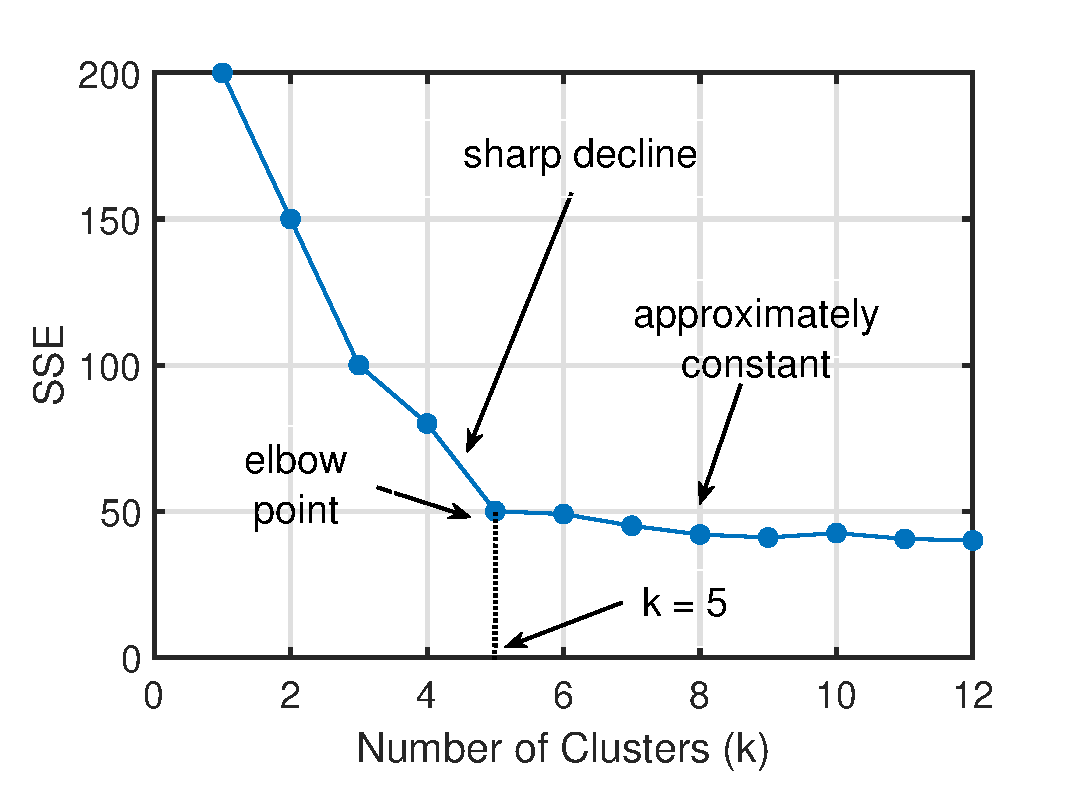
\includegraphics[width=0.45\textwidth]{elbow_ideal.eps}}
        }
        \mbox{
            \subfigure[Método da Silhueta.]{
            \label{fig:silhouete-ideal}
            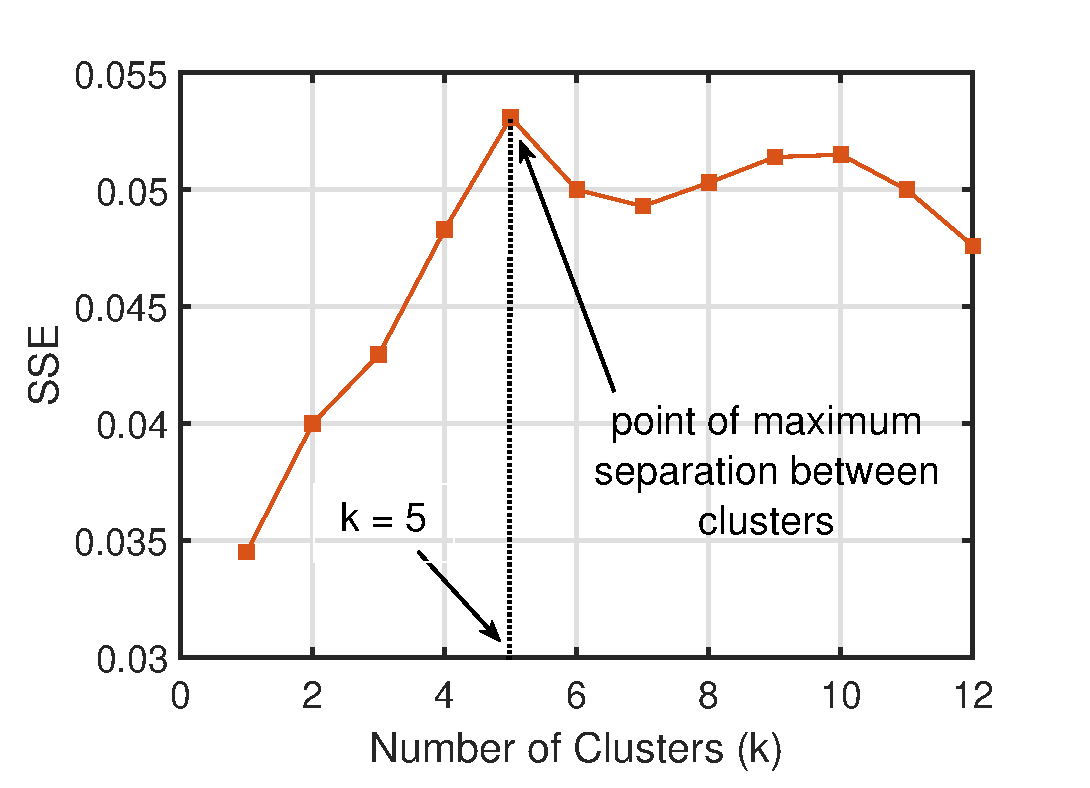
\includegraphics[width=0.45\textwidth]{silhouette_ideal.eps}}
        }
    \end{center}
    \caption{Métodos complementares para determinar o número ótimo de agrupamentos. Ambos os métodos idealmente tendem a convergir para um mesmo k, verificado neste exemplo como k=5.}
    \label{fig:elbow_silhouette_ideal}
\end{figure}

Contudo ambos os algoritmos, assim como outros, estão sujeitos à uma desvantagem singular: a indeterminação quanto ao número adequado de grupos $k$. A fim de contornar essa indeterminação, são usados dois métodos, do Cotovelo (\textit{Elbow}) e da Silhueta (\textit{Silhouette}), para analisar previamente a conformidade dos dados a quantidades diferentes de grupos e, assim, obter um resultado adequado aos dados. Em particular, o método do Cotovelo mede a compactação dos agrupamentos estabelecendo uma relação entre o número de agrupamentos e sua influência na variação total dos dados dentro do grupo. Graficamente, o melhor valor de $k$ é encontrado identificando o ponto em que o ganho da curva diminui drasticamente, permanecendo aproximadamente constante depois disso. De forma análoga, o método da Silhueta mede a qualidade de um agrupamento. O número ideal de agrupamentos $k$ é aquele que maximiza a silhueta média em uma faixa de valores possíveis para $k$ \cite{ketchen1996application,rousseeuw1990finding}. A Figura~\ref{fig:elbow_silhouette_ideal} mostra um exemplo hipotético de uso dos métodos do Cotovelo e da Silhueta. Nesse exemplo hipotético, é visto que para o valor $k=5$ há uma mudança brusca no erro médio quadrático (SSE) interno aos agrupamentos no método do Cotovelo e, para $k=5$, também há um ponto máximo do erro médio quadrático entre os agrupamentos no método da Silhueta, indicando maior separação entre agrupamentos.



Ressalta-se ainda que há variações dos algoritmos \textit{k-means} e \textit{k-medoids} que consideram graus de pertinência de uma amostra a diversos grupos. Nesses casos, chamados \textit{fuzzy k-means} e \textit{fuzzy k-medoids}, o centro dos agrupamentos são calculados considerando a pertinência parcial de cada amostra aos agrupamentos.

\subsubsection{Algoritmos Baseados em Densidade}
\label{subsubsec:densidade}

Algoritmos de agrupamento baseados em densidade compartilham uma relação próxima com a abordagem do vizinho mais próximo (\textit{nearest neighbour}). Nesse sentido, um agrupamento, definido como um componente denso conectado, cresce em qualquer direção que a densidade o conduza. Essa lógica de formação dos agrupamentos está diretamente relacionada à principal vantagem desses algoritmos em relação ao grupo dos algoritmos de particionamento, a possibilidade de descobrir agrupamentos com formas arbitrárias, diferente dos agrupamentos tipicamente esféricos retornados pelo algoritmo \textit{k-means}, por exemplo.

Dentre os algoritmos baseados em densidade, o algoritmo de \textbf{Clusterização Espacial Baseada em Densidade de Aplicações com Ruído} (\textit{Density Based Spatial Clustering of Application with Noise} -- DBSCAN) é o mais popular. Seu intuito é encontrar regiões que satisfaçam uma densidade de pontos mínima estabelecida e que sejam separadas por regiões de menor densidade. Para isso, o algoritmo realiza uma estimativa simples do nível de densidade mínimo, definindo um limite para o número de vizinhos, $minPts$, dentro de um raio $\epsilon$. Assim, uma amostra 
com mais de $minPts$ vizinhos dentro desse raio, é considerada um ponto central. Analogamente, uma amostra é considerada como de borda, se dentro de sua vizinhança concentram-se menos amostras que o mínimo definido, porém a amostra ainda pertence à vizinhança de um ponto central qualquer. Por último, amostras que não são alcançáveis por densidade a partir de qualquer ponto central, ou seja, não se configuram nem como pontos centrais nem de borda, são rotulados como \textit{outliers}. Uma desvantagem associada ao seu uso consiste na sua complexidade fortemente polinomial, que requer $\Omega (n^{\frac {4}{3}})$ tempo para convergir, em que $ n $ é o tamanho do conjunto de dados~\cite{fahad2014survey, gan2015dbscan, schubert2017dbscan}.

\subsubsection{Algoritmos Hierárquicos}
\label{subsubsec:hierarquico}

Os algoritmos hierárquicos não apenas criam agrupamentos, mas consideram uma lógica multinível e calculam uma representação hierárquica dos dados de entrada. Esta representação é um tipo particular de árvore, em que os nós-folhas expressam dados individuais, e pode ser construída seguindo um método aglomerativo ou divisivo. O método aglomerativo, conhecido também como abordagem \textit{bottom-up}, começa considerando cada amostra como um agrupamento unitário e mescla recursivamente duas ou mais em um novo agrupamento seguindo uma função de ligação escolhida. Tais funções, quando associados à métricas de distância ou de similaridade, definem critérios únicos que elegem os agrupamentos mesclados de cada iteração. A função de ligação única (\textit{single-linkage}), por exemplo, estabelece a união considerando a distância entre as amostras mais próximos de cada agrupamento. De forma oposta, a função de ligação completa (\textit{complete-linkage}) considera a distância das amostras mais distantes entre si cada agrupamento. Paralelamente, a função de ligação média (\textit{average linkage}) calcula a média das distâncias de todas as amostras de um agrupamento em relação a todas as amostras de outro agrupamento. Em especial, o critério de Ward emprega a distância euclidiana na descoberta do par de agrupamentos que minimizam o aumento na variância total interna após a união.

\begin{figure}[ht]
    \begin{center}
        \mbox{
            \subfigure[Critérios de Ligação do Método Aglomerativo]{
            \label{fig:linkage}
            \includegraphics[width=0.5\textwidth]{linkage.png}}
        }
        \mbox{
            \subfigure[Dendrograma]{
            \label{fig:dendrograma}
            \includegraphics[width=0.43\textwidth]{dendograma2.png}}
        }
    \end{center}
    \caption{(a) Representação bidimensional de diferentes critérios de ligação da considerando 6 amostras já alocadas em dois agrupamentos. b) Dendrograma resultante da aplicação do algoritmo de agrupamento hierárquico sobre as amostras 1-6. O algoritmo emprega o método aglomerativo usando critério de ligação única.}
    \label{fig:hiearquico}
\end{figure}

Por outro lado, o método divisivo, e.g. abordagem \textit{top-down}, inicia com uma estrutura plana em que todas as amostras pertencem ao mesmo agrupamento, ou seja, nível hierárquico. Portanto, a cada iteração, o algoritmo divide um ramo-pai em dois subconjuntos menores, os ramos-filhos. O processo termina quando um critério de parada é atingido, frequentemente, o número $ k $ de agrupamentos. No final do algoritmo, é criado um dendrograma de agrupamentos, uma hierarquia de árvore binária~\cite{benavent2019fca, icnc-2020-nicollas, fahad2014survey, govender2020application}. Um possível agrupamento hierárquico considerando a disposição espacial entre as amostras 1-6 da Figura \ref{fig:linkage}
é ilustrada na Figura~\ref{fig:dendrograma}. Traçando as retas pontilhadas A-D perpendiculares aos ramos verticais do dendrograma é possível identificar diferentes momentos do processo de agrupamento. Em $A$, nota-se a existência de 6 agrupamentos unitários, ou seja, cada um contendo as amostras. Em $B$, constata-se a existência de 3 agrupamentos: o agrupamento unitário da amostra 1, o agrupamento das amostras 2 e 3, além do agrupamento formado pelas amostras 4, 5 e 6. Em $C$, 
já é possível identificar o mesmo par de agrupamentos retratados na Figura \ref{fig:linkage}. Por fim, em $D$ verificamos a presença de um único agrupamento superpopuloso, contendo todas as amostras iniciais. 

\subsection{Métricas de Avaliação}
\label{subsec:metricasdeavaliação}

Independente do algoritmo, supervisionado ou não-supervisionado, caso haja o conhecimento prévio sobre dados rotulados com base em uma verdade básica (\textit{ground truth}), torna-se plausível a clara identificação de quantidade de Verdadeiros Positivos (VP), Falsos Positivos (FP), Verdadeiros Negativos (VN) e Falsos Negativos (FN). Tais classificações compõem o cálculo de várias métricas de recuperação de informação, resumidas na Figura~\ref{fig:metricas_roc}, como:
\begin{itemize}
    \item \textbf{Acurácia} ($A_c$) é definida pela razão do total de amostras classificadas corretamente (VP + VN), pelo número total de amostras (P+N). Para conjunto de dados não-balanceados, uma avaliação de desempenho baseada exclusivamente nesta métrica pode gerar conclusões erradas;
    \item \textbf{Precisão} ($P_r$) é a razão entre, dada uma classe alvo, a quantidade de amostras corretamente classificadas para a classe em questão (VP), pelo conjunto total de predições atribuídas a essa classe, isto é, corretas e incorretas (VP + FP);
    \item \textbf{Sensibilidade} ($S_s$) também conhecida como revocação (\textit{recall}) ou \textbf{taxa de verdadeiros positivos} é definida pela razão entre a quantidade de amostras corretamente preditas (VP) para um classe positiva e o total de amostras que pertencem a esta classe, incluindo assim tanto predições corretas quanto as que deveriam ter indicado esta classe (VP + FN). O análogo para a classe negativa é chamado de \textbf{especificidade} ou \textbf{taxa de verdadeiros negativos};
    \item \textbf{Medida-$F_{1}$} (\textit{$F_{1}$-Score}) relaciona a precisão e a sensibilidade por uma média harmônica expressa por 
\begin{equation}
    Medida-F_{1} = \frac{2}{\frac{1}{P_{r}}+\frac{1}{S_{s}}};
\end{equation}
    Geralmente, quando maior o valor da medida-$F_{1}$, melhor a classificação sendo um reflexo do compromisso mútuo entre a precisão ($P_r$) a sensibilidade ($S_s$): 
\end{itemize}

\begin{itemize}
    \item \textbf{Área abaixo da curva ROC} é medida através da curva Característica de Operação do Receptor (ROC), mostrada na Figura~\ref{fig:_ideal}, uma representação da razão entre a taxa de verdadeiros positivos (TPR) e a taxa de falsos positivos (FPR), para vários limiares de corte. Essa curva descreve graficamente o desempenho de um modelo de classificação. Sucintamente, quanto maior a área abaixo da curva (mais próxima ao valor unitário), melhor o desempenho do modelo, independentemente do ponto de corte da probabilidade de pertencimento de à classe de cada amostra. 
\end{itemize}

\begin{figure}[ht]
    \begin{center}
        \mbox{
            \subfigure[Curvas ROC de Classificadores]{
            \label{fig:_ideal}
            \includegraphics[width=0.40\textwidth]{roc_ideal.png}}
        }
        \mbox{
            \subfigure[Métricas de Recuperação da Informação]{
            \label{fig:metricas}
            \includegraphics[width=0.5\textwidth]{metricas.png}}
        }
    \end{center}
    \caption{(a) Curvas ROC de classificadores e comparação da área abaixo da curva ROC (\textit{Area Under the Curve}, AUC). b) Ilustração das métricas acurácia, precisão e sensibilidade em um problema de classificação binária.}
    \label{fig:metricas_roc}
\end{figure}



\section{As Soluções para Processamento de Dados em Linguagem Natural em Nuvens Comerciais}
\label{sec:solucoes-nuvem}


% Apresentar as duas abordagens de AI Services e AI Platform, seus públicos-alvo e listar as opções na AWS, Azure e GCP.
Para implementar as diferentes técnicas e algoritmos apresentados em plataformas de computação em nuvem é preciso levar em consideração o tipo de atividade que se espera que o provedor de serviço na nuvem entregue. Os principais provedores de serviço na nuvem públicos são a Amazon Web Service (AWS), a Microsoft Azure e o Google Cloud Platform (GCP). Cada um desses provedores de nuvem oferecem infraestrutura mais simples, como entidades de recursos computacionais análogos a máquinas virtuais, plataformas completas de desenvolvimento, como plataformas que gerenciam a criação de recursos computacionais análogos a máquinas virtuais, até serviços computacionais específicos que não dependem que os usuários gerenciem a infraestrutura de forma alguma, funcionando através de requisições \textit{web} através do protocolo HTTP.

Serviços de inteligência artificial seguem padrão semelhante aos recursos de nuvem em geral, nos quais cada tipo desses recursos tem como público alvo um segmento de profissionais. As plataformas de nuvem dividem a abordagem na qual irão disponibilizar suas ofertas em três camadas: Plataformas de Inteligência Artificial (\textit{Artificial Inteligence Services}), Serviços de Inteligência Artificial (\textit{Artificial Inteligence Platforms}) e Motores de Inteligência Artificial (\textit{Artificial Inteligence Engines}). As próximas subseções detalham  cada uma destas três camadas, suas peculiaridades, precificação e público alvo.


\subsection{Plataformas de Inteligência Artificial}

As plataformas de inteligência artificial~\footnote{Disponíveis em https://aws.amazon.com/pt/machine-learning/ai-services/.}, chamadas de \textit{AI Platforms}, estão relacionados com a utilização de alguma solução que facilita o ciclo de vida de uma aplicação de inteligência artificial. As \textit{AI Platforms} oferecem o gerenciamento de infraestrutura necessário para treinar e disponibilizar modelos de inteligência artificial e também para fazer a engenharia de características (\textit{feature engineering}) dos dados e lidar com predições em tempo real utilizando algoritmos implementados em estrutura de computação distribuída, como oferecidas pelo arcabouço Apache Spark em sua biblioteca \texttt{MLlib}~\footnote{Disponível em https://spark.apache.org/mllib/.}. Esses serviços exigem conhecimento prévio dos algoritmos de inteligência artificial, visto que eles devem ser implementados e o modelo deve ser treinado com dados fornecidos. As \textit{AI Platforms} apoiam esse processo, oferendo recursos para gerenciar o treinamento e a implantação dos modelos, nos quais a implantação de um modelo treinada é realizada em menos de 5 minutos\footnote{A implantação do modelo treinado se refere ao processo de construção de uma aplicação que utiliza o modelo treinado, recebendo requisições HTTP com os dados de entrada e retornando o resultado da predição do modelo}.

No caso especifico de uma solução de extração de entidades de um texto, o usuário deverá escolher o algoritmo adequado para solucionar o problema em questão, usar a plataforma oferecida pelas \textit{AI Platforms} para auxiliar na ingestão de dados de forma segura, transformação dos dados e engenharia de características, utilizar as ferramentas para controle e gerência do treinamento dos dados, que pode ser realizada com uma estrutura de recursos computacionais totalmente apartada, com CPU e  GPU dedicadas para aquele treinamento, e, por fim, utilizar o serviço que recebe o modelo treinado e cria a infraestrutura juntamente com o servidor HTTP responsável por receber as requisições e retornar as predições.

Os provedores precificam esses serviços com base na quantidade de recurso computacional utilizadas por hora e pela quantidade de armazenamento utilizada, em que alguns deles, como o Amazon Sagemaker na AWS\footnote{Disponível em https://aws.amazon.com/pt/sagemaker/.}, costumam cobrar uma taxa a mais pelo uso da plataforma em si. Esse modelo de cobrança otimiza o uso de recursos, tendo em vista a possibilidade da utilização de recursos computacionais como GPUs em um modelo de aluguel por hora, não necessitando de investimento inicial.

Serviços de \textit{AI Platforms} são recomendados para cientistas de dados e engenheiro de aprendizado de máquina que necessitam implantar aplicações específicas implementando o ciclo completo de desenvolvimento dos modelos, desde a extração dos dados até o monitoramento do modelo final implantado.

\subsection{Serviços de Inteligência Artificial}

Os serviços de inteligência artificial~\footnote{Disponíveis em https://aws.amazon.com/pt/machine-learning/ai-services/.}, chamados de \textit{AI Services}, estão relacionados com a utilização de alguma solução de inteligência artificial implementada previamente pelo provedor de serviço em nuvem. Essas soluções são baseadas em soluções de problemas específicos, como a transformação de texto em voz ou para realizar processamento de linguagem natural extraindo entidades de textos. Esses serviços não exigem conhecimento prévio dos algoritmos de inteligência artificial. Entre os serviços mais comuns estão a automatização de revisões de códigos, a criação de \textit{chatbots}, prevenção de fraudes, traduções em tempo real, transcrição e sintetização de fala, entre outros.

Essa categoria de serviços não exige que os usuários treinem os modelos. A utilização é baseada em requisições através do protocolo HTTP, nas quais o usuário envia os dados específicos para a predição e o provedor de serviços na nuvem executa a predição e retorna o resultado. No caso específico de uma solução de extração de entidades de um texto, o usuário deve enviar o texto para o provedor, o provedor analisará o texto com seu modelo proprietário e retornará as entidades encontradas. Por questão de privacidade dos dados, os provedores não armazenam os dados fornecidos pelos usuários ao realizar as predições.

Os provedores precificam esses serviços com base na quantidade de dados que são utilizados como entrada para as predições e a quantidade de requisições feitas pelos usuários. Essa relação de cobrança acarreta que o custo de execução pode ficar mais elevado do que se o usuário realizasse as predições nos próprios modelos. Contudo, o custo é compensado pelo fato do usuário não precisar criar, treinar e gerenciar esses modelos.

Os \textit{AI Services} são recomendados quando o usuário não tem experiência implementando seus próprios algoritmos de inteligência artificial ou para resolução de problemas clássicos e específicos que o provedor já forneça solução pronta que satisfaz os requisitos para a resolução do problema. Os \textit{AI Services} levam a resultados imediatos mediante as requisições \textit{web} através do protocolo HTTP. 

\subsection{Motores de Inteligência Artificial}

Os motores de inteligência artificial, chamados de \textit{AI Engines}, são a camada dedicada ao uso direto, sem intermédio de uma solução do provedor de serviço em nuvem, de arcabouços de código aberto, como Apache MXNet, Tensorflow e Torch, provendo flexibilidade total aos cientistas de dados e engenheiros de aprendizado de máquina para testar novas implementações de algoritmos, sistemas mais sofisticados que exigem algum recurso de mais baixo nível, como o uso de C e C++. Em geral, é a escolha de pesquisadores que estão implementando um novo modelo otimizado e precisam de total liberdade do sistema operacional, não dependendo de nenhuma implementação prévia do provedor de serviços em nuvem.

Esses serviços funcionam com o provisionamento da infraestrutura requerida pelo usuário para execução do desenvolvimento, treinamento e implantação do modelo. Recursos de GPU, CPU, chegando até mesmo ao nível mais específico de \textit{Field-Programmable Gate Arrays} (FPGAs). Nessa categoria de serviço os provedores de serviço em nuvem alugam recursos computacionais análogos a máquinas virtuais para os usuários.

Os provedores precificam esses serviços analogamente às \textit{AI Platform}, exceto pelo custo extra de licença para a utilização de algumas plataformas em particular.
\textit{AI Platforms} são recomendadas para cientistas de dados e engenheiro de aprendizado de máquina que precisam escrever aplicações do zero, com total liberdade de escolha de qualquer tipo de arcabouço e linguagem de programação, com a desvantagem de ter que gerenciar a infraestrutura total requisitada, enquanto \textit{AI Engines} são recomendados para usuários que possam utilizar os arcabouços específicos já implantados na nuvem.


% Para Processamento de linguagem natural, explicar como funcionam  cada uma das soluções tomando a AWS como exemplo
%--

% Em cada solução, apresentar vantagens e desvantagens e estrutura de custo.
%--


\section{As Iniciativas de Pesquisa}
\label{sec:pesquisa}

Diversas atividades de pesquisa estão ativas e buscam caracterizar e mitigar os desafios causados pelas notícias falsas.
Uma definição inicial sobre as notícias falsas é feita por Lazer \textit{et al.}. No artigo, é abordada a historia das notícias falsas começando pela difamação na Primeira Guerra Mundial até o impacto das notícias falsas durante a eleição presidencial dos Estados Unidos em 2016~\cite{lazer2018science}. Grinberg \textit{et al.} aprofundam no impacto das notícias falsas durante as eleições de 2016, analisando as mensagens da rede social \textit{Twitter}~\cite{grinberg2019fake}. Os autores coletaram \textit{tweets} enviados por 16.442 contas ativas durante a temporada eleitoral de 2016, de 1º de agosto até 6 de dezembro de 2016. Os resultados mostram que os grupos de maior idade, entre 60 e 80 anos, com afinidade politica de direita ou extrema direita são mais propensos à distribuição e ao compartilhamento de notícias políticas falsas. A recente pandemia da Doença Infecciosa por Corona Vírus de 2019 (COVID-19) também é um evento no qual foram disseminadas grande quantidade de notícias falsas. Estudos recentes mostram a correlação entre o uso de mídia social e a desinformação durante a pandemia~\cite{pennycook2020fighting, van2020using}.  

A detecção de notícias falsas é estudada sob várias perspectivas como Aprendizado de Máquina, Mineração de Dados e Processamento de Linguagem Natural. O Saco-de-Palavras e as frequências de categorias são utilizadas para  o treinamento de classificadores como as Máquinas de Vetores Suportes (\textit{Support Vector Machines } - SVM) e modelos bayesianos ingênuos~\cite{poddar2019comparison}. Uma vez que o modelo matemático é treinado a partir de exemplos conhecidos das duas categorias, notícia falsa ou não, é possível prever instâncias futuras com base em agrupamento numérico e distâncias. O uso de diferentes métodos de agrupamento e funções de distância entre os pontos de dados é uma das bases do algoritmo do SVM. Por outro lado, o algoritmo bayesiano ingênuo faz classificações com base em evidências acumuladas da correlação entre uma determinada variável, como a sintaxe, e as outras variáveis presentes no modelo.

Shu \textit{et al.} fazem uma revisão da detecção de notícias falsas nas mídias sociais de uma perspectiva de mineração de dados, incluindo caracterização de notícias falsas sobre psicologia e teorias sociais, algoritmos existentes, métricas de avaliação e conjuntos de dados representativos~\cite{shu2017fake}. \textit{Fake News Tracker} é uma solução para coleta de dados, visualização interativa e modelagem analítica para detecção de notícias falsas. A solução utiliza técnicas de Processamento de Linguagem Natural~\cite{shu2019fakenewstracker}. 

Alguns trabalhos apresentam técnicas e desafios sobre a detecção de notícias falsas. Zhou e Zafarani identificam e detalham as teorias fundamentais relacionadas em diferentes disciplinas para a detecção de notícias falsas~\cite{zhou2018fake}. Sharma \textit{et al.} discutem os métodos e técnicas existentes aplicáveis à identificação e à mitigação de notícias falsas, com foco nos avanços significativos em cada método e suas vantagens e limitações~\cite{sharma2019combating}. Bondielli e Marcelloni fazem um levantamento da literatura sobre as diferentes abordagens para a detecção automática de notícias falsas e rumores~\cite{BONDIELLI201938}. Os autores destacam várias abordagens adotadas para coletar dados de notícias falsas e rumores. 

Oshikawa \textit{et al.} apresentam uma comparação dos métodos usados na detecção de notícias falsas usando Processamento de Linguagem Natural (PLN)~\cite{oshikawa2018survey}. De forma semelhante, Sharma \textit{et al.} analisam a revisão da literatura sobre PLN aplicado em notícias falsas, ressaltando a comparação entre as diferentes técnicas de aprendizado de máquina, aprendizado profundo e outras técnicas~\cite{sharma2019combating}. Deepak and Chitturi compararam diferentes tipos de redes neuronais na detecção de notícias falsas~\cite{deepak-lstm}. Feng \textit{et al.} propõem uma rede neural convolucional de dois níveis com gerador de resposta do usuário, em que a rede neural captura informações semânticas do texto, representando-as no nível de frase e de palavra, e o gerador de resposta de usuário aprende um modelo da resposta do usuário ao texto da notícia~\cite{fengAndSharma}. 


% definition
% https://www.tandfonline.com/doi/full/10.1080/21670811.2017.1360143?scroll=top&needAccess=true

% surveys

% https://www.pnas.org/content/pnas/116/16/7662.full.pdf
% https://arxiv.org/pdf/1812.00315.pdf
% https://dl.acm.org/doi/pdf/10.1145/3289600.3291382?casa_token=kqo_C2LbUlEAAAAA:E4Nq2-EEpAmvSdtIbxt6ZZbXRlhd86f_sqiohFtWo09Bzvz3tu5d_676sVrHfrFaI8Ntu8i13ACE
% https://dl.acm.org/doi/pdf/10.1145/3377330.3377334?casa_token=lNBcZUFGRuIAAAAA:mVMmVItRoPLuxK1DqxP8tiRhXyqVcrJfjuMvVztT7NyvuulMiSFmYVJbhCOilfwTb2CdQ9MjY9bF
% http://pike.psu.edu/publications/abs19.pdf
% https://philpapers.org/archive/PEPWNA.pdf
% https://onlinelibrary.wiley.com/doi/abs/10.1111/soc4.12724
% http://www.andrewtlittle.com/papers/little_fakenews_cp.pdf
% https://www.sciencedirect.com/science/article/abs/pii/S016792362030035X
% http://sbp-brims.org/2018/proceedings/papers/challenge_papers/SBP-BRiMS_2018_paper_116.pdf
% https://commons.emich.edu/cgi/viewcontent.cgi?article=1322&context=loexquarterly
% https://dspace.lib.uom.gr/bitstream/2159/23448/4/RaptiMatinaMsc2019.pdf
% https://www.sciencedirect.com/science/article/pii/S2352250X20300439
% https://www.researchgate.net/profile/Xinyi_Zhou26/publication/342762209_A_Survey_of_Fake_News_Fundamental_Theories_Detection_Methods_and_Opportunities/links/5f1644f9a6fdcc3ed71b23cd/A-Survey-of-Fake-News-Fundamental-Theories-Detection-Methods-and-Opportunities.pdf

% covid 
% https://www.researchgate.net/profile/Beatriz_Villarejo/publication/340658737_COVID-19_infodemic_More_retweets_for_science-based_information_on_coronavirus_than_for_false_information/links/5e99749c299bf13079a203b8/COVID-19-infodemic-More-retweets-for-science-based-information-on-coronavirus-than-for-false-information.pdf
% https://www.ncbi.nlm.nih.gov/pmc/articles/PMC7202120/
% https://arxiv.org/pdf/2007.09682
% https://www.ncbi.nlm.nih.gov/pmc/articles/PMC7390799/


% us election
% https://dl.acm.org/doi/pdf/10.1145/3308558.3313721?casa_token=jLo5nde502UAAAAA:S6SpC1qIVkMjWIJdLFFd8Ux5sTZsqfeWOaj6XP9yhdSY0nkr0qDIhOc1vmzpVXivHijj85dmYYs5
% https://www.nber.org/papers/w23089.pdf
% http://www.ask-force.org/web/Fundamentalists/Guess-Selective-Exposure-to-Misinformation-Evidence-Presidential-Campaign-2018.pdf

% data mining
% http://www.vldb.org/pvldb/vol12/p1990-lakshmanan.pdf


% model
% https://apps.dtic.mil/dtic/tr/fulltext/u2/1061567.pdf
% https://dl.acm.org/doi/pdf/10.1145/3377478

% portuguese and detection
% https://www.sciencedirect.com/science/article/abs/pii/S0957417420300257
% https://arxiv.org/pdf/1705.00648.pdf
% https://asistdl.onlinelibrary.wiley.com/doi/pdf/10.1002/pra2.2015.145052010083
% https://asistdl.onlinelibrary.wiley.com/doi/pdf/10.1002/pra2.2015.145052010082

% facebook
% https://advances.sciencemag.org/content/5/1/eaau4586.full

% social bots
% https://www.andyblackassociates.co.uk/wp-content/uploads/2015/06/fakenewsbots.pdf

% NLP
% https://sci-hub.st/https://ieeexplore.ieee.org/abstract/document/8665593
% https://www.sciencedirect.com/science/article/abs/pii/S095741741930661X

% machine learning
% https://www.researchgate.net/profile/Marina_Ibrishimova/publication/335191041_A_Machine_Learning_Approach_to_Fake_News_Detection_Using_Knowledge_Verification_and_Natural_Language_Processing/links/5dd0b7db299bf1b74b48ac28/A-Machine-Learning-Approach-to-Fake-News-Detection-Using-Knowledge-Verification-and-Natural-Language-Processing.pdf

\section{Desafios e Oportunidades de Pesquisa}
\label{sec:desafios}

Embora as pesquisas na identificação, detecção e mitigação da propagação de notícias falsas estejam em pelo desenvolvimento, alguns dos principais desafios no combate às notícias falsas são listados a seguir~\cite{sharma2019combating}.

\begin{itemize}

\item {\bf Grandes interesses e a pluralidade de atores envolvidos.} Devido ao volume que a propagação de notícias falsas atinge em redes sociais em um período curto, as notícias falsas representam uma ameaça às fontes tradicionais de informações, como a impressa tradicional. O espalhamento de notícias falsas ocorre como um evento distribuído e, então, envolve múltiplas entidades e plataformas tecnológicas. Assim, há uma crescente dificuldade de estudar e projetar estratégias computacionais, tecnológicas e de negócios de combate às notícias falsas sem que haja o comprometimento da rapidez e do acesso colaborativo a informações de alta qualidade.

\item {\bf Intenção maliciosa do adversário.} O conteúdo das notícias falsas é projetado para dificultar a identificação por humanos das notícias falsas, explorando suas habilidades cognitivas, emoções e preconceitos ideológicos. Além disso, é desafiador para métodos computacionais detectar notícias falsas, pois a forma como as notícias falsas são apresentadas é semelhante à de notícias verídicas e, por vezes, as notícias falsas usam artifícios para dificultar a identificação da fonte ou falsificam a verdadeira fonte da notícia.

\item {\bf Suscetibilidade e falta de conscientização do público.} O usuário de redes sociais está sujeito a uma grande quantidade de informações de origens duvidosas, desde informações com cunho humorístico, como sátiras, até informações com o intuito de enganar o consumidor de informações se passando por notícias verídicas. Contudo, o usuário de redes sociais não é capaz de diferenciar uma notícia falsa de uma verídica apenas pelo conteúdo. O usuário não dispõe de informações sobre a credibilidade da fonte ou padrões de propagação da notícia na rede. Assim, para aumentar a conscientização pública, vários artigos e campanhas publicitárias são veiculados para fornecerem dicas sobre como diferenciar notícias verídicas de falsas. Por exemplo, a Universidade de Portland, nos Estados Unidos, disponibiliza um guia para a identificação de desinformação (notícias falsas)\footnote{Disponível em https://guides.library.pdx.edu/c.php?g=625347\&p=4359724.}. 

\item {\bf Dinâmica de propagação.} A propagação de notícias falsas em mídia social complica a detecção e a mitigação, pois as informações falsas podem facilmente alcançar e afetar um grande número de usuários em pouco tempo. A informação é transmitida de maneira rápida e fácil, mesmo quando sua veracidade é duvidosa~\cite{friggeri2014}. A verificação da veracidade deve ser realizada de forma ágil, mas também deve considerar os padrões de propagação da informação ao longo da rede~\cite{meel2020}.

\item {\bf Mudanças constante das características das notícias falsas.} Os desenvolvimentos na identificação automatizada de notícias falsas também impulsionam a adaptação da geração de novos conteúdos de desinformação para evitarem de serem classificados como tal. A detecção de notícias falsas baseada em estilo de escrita, diferenciando notícias falsas e verdadeiras por uma análise baseada no processamento de linguagem natural, é uma das principais alternativas usadas devido aos desafios não resolvidos na automatização da verificação de fatos a partir de bases de conhecimento pré-definidas. Assim, abordagens atuais de identificação de notícias falsas baseadas no conteúdo focam na extração de fatos diretamente do conteúdo da notícia e a posterior verificação dos fatos contra bases de conhecimento~\cite{ciot-nicollas-2020}.

\item {\bf Ataques ao aprendizado por linguagem natural.} Zhou {\it et al.} argumentam que o uso de processamento de linguagem natural para a identificação de notícias falsas é vulnerável a ataques ao aprendizado de máquina em si~\cite{zhou-arxiv}. Zhou {\it et al.} identificam três ataques: a distorção de fatos, a troca entre sujeito e objeto; e a confusão de causas. A distorção de fato consiste em exagerar ou modificar algumas palavras. Elementos textuais, como personagens e tempo, podem ser distorcidos para levar a uma interpretação falsa. A troca entre sujeito e objeto tem como objetivo confundir o leitor entre quem pratica e quem sofre a ação relatada. O ataque de confusão de causa consiste em criar relações causais inexistentes entre dois eventos independentes ou cortar partes de uma história, deixando apenas as partes que o atacante deseja apresentar para o leitor~\cite{zhou-arxiv}.

\end{itemize}

As oportunidades de pesquisa na identificação e mitigação de notícias falsas focam na detecção rápida ou em tempo real da fonte, no controle da propagação das informações falsas e na redução do impacto das notícias falsas na sociedade. Conjuntos de dados coletados em tempo real, detecção automática de rumores e localização da fonte original são questões de pesquisa desafiadoras~\cite{meel2020}. A seguir destacam-se as principais oportunidades de pesquisa e desenvolvimento de soluções para o combate às notícias falsas.

\begin{itemize}
    \item {\bf Extração de características mais significativas.} Determinar as características mais eficazes para detectar notícias falsas de múltiplas fontes de dados é uma oportunidade de pesquisa em aberto. Fundamentalmente, existem duas fontes de dados principais: o conteúdo das notícias e contexto social~\cite{shu2017fake}. Da perspectiva de conteúdo de notícias, técnicas baseadas em processamento de linguagem natural e extração de características podem ser usadas para extrair informações do texto. Técnicas de incorporação, como incorporação de palavras (\textit{word embedding}) e redes neurais profundas são foco de pesquisas atuais para a extração de características textuais e têm o potencial para aprender melhores representações para os dados. Características visuais extraídas das imagens também são indicadores importantes para notícias falsas. O uso de redes neurais profundas é uma oportunidade de pesquisa na extração de características visuais para a detecção de notícias falsas~\cite{sharma2019combating,meel2020}.

    \item {\bf Detecção em diferentes plataformas e diferentes domínios.}  Devido ao fato dos usuários utilizarem diferentes redes sociais, as notícias falsas e boatos se espalham nas diferentes plataformas, dificultando a localização da origem da notícia ou do boato. O rastreamento da origem da informação falsa entre plataformas distintas de redes sociais é uma oportunidade de pesquisa. Para tanto, devem ser considerados diversos aspectos da informação. Contudo, a maior parte da abordagem existente se concentra apenas em uma das formas de detecção da informação falsa: análise de conteúdo, da propagação, do estilo, entre outras. A análise deve considerar, então, diferentes domínios de atributos, como tópicos, sítios \textit{web}, imagens e URLs~\cite{meel2020}.

    \item {\bf Identificação de câmaras de eco e ponte entre as câmaras.}  A mídia social tende a formar câmaras de eco em comunidades em que usuário têm visões e ideologias semelhantes. Os usuários têm suas visões reforçadas e não estão cientes das crenças opostas. Portanto, pesquisas são necessárias para identificar câmaras de eco conflitantes e ligar as câmaras com posições opostas para que os usuários sejam confrontados com visões distintas. Isso também ajuda na descoberta da verdade, fazendo os usuários pensarem criteriosamente e racionalmente em múltiplas dimensões~\cite{meel2020}.

    \item {\bf Desenvolvimento de modelos de aprendizado de máquina.} Há a necessidade de pesquisa no desenvolvimento de modelos de aprendizado em tempo real, tais como aprendizado incremental e aprendizado federado, capazes de aprender com artigos verificados manualmente e fornecer detecção em tempo real de novos artigos com informações fraudulentas. Outro ponto importante é o desenvolvimento de modelos não-supervisionados em que os algoritmos aprendem com dados reais e, então, artigos que fogem do comportamento de dados reais são classificados como falsos. Há ainda uma escassez de conjuntos de dados específicos para notícias falsas. A falta de conjuntos de dados de larga escala publicamente disponíveis implica a carência de testes (\textit{benchmarks}) para a comparação de desempenho entre algoritmos diferentes~\cite{meel2020}.


    \item {\bf Desenvolvimento de estruturas de dados capazes de lidar com a estrutura de rede complexa e dinâmica.}  A complexidade e a dinamicidade das estruturas de relacionamento em redes sociais tornam a tarefa de identificação e rastreamento de publicações mais complicadas. Assim, há a necessidade de pesquisa para o desenvolvimento de estruturas de dados complexas que reflitam a dinamicidade das relações em redes sociais para permitir a extração de conhecimento acerca da propagação de informações falsas na rede~\cite{meel2020}.

\end{itemize}

\section{Atividade Prática}
\label{sec:pratica}

Esta seção consolida a uma pluralidade de conceitos teóricos abordados no capítulo através de uma atividade prática do processo de identificação de notícias falsas em redes sociais, empregando a linguagem \texttt{Python}. O processo ocorre na rede social \textit{Twitter} e é representado na Figura~\ref{sec:pratica}. O processo inclui (i) a coleta de notícias, falsas e verdadeiras, empregando a interface de programação de aplicação (\textit{Application Programming Interface} - API) do \textit{Twitter} para efetuar o \textit{web scraping}\footnote{Também conhecida como coleta, ou raspagem de dados, é uma forma de mineração capaz de extrair o conteúdo de sítios da \textit{web} para uma posterior análise.}; (ii) o processamento textual e vetorização do conteúdo das notícias, empregando PLN juntamente com técnicas de representação vetorial de textos; (iii) a aplicação eficiente de algoritmos de detecção, alcançado pela incorporação de técnicas de redução de dimensionalidade; e (iv) a avaliação da eficiência e qualidade da detecção, tendo como parâmetros as métricas de recuperação de informação.

\begin{figure}[h]
	\centering
	\includegraphics[width=.9\columnwidth]{pratica.png}
	\caption{Fluxograma do processo de identificação de notícias falsas desenvolvido na atividade prática. A primeira etapa compreende a formação da base de dados formada por notícias falsas e legítimas. Na segunda etapa são aplicadas técnicas de processamento de linguagem natural e vetorização. Na terceira etapa, após uma redução dimensional, a representação vetorial das notícias é submetida a algoritmos de detecção. A quarta etapa concentra-se em avaliar a qualidade da detecção segundo métricas de recuperação de informação.}
	\label{fig:pratica}
\end{figure}

Como primeira etapa da atividade prática, a composição da base de dados inclui tanto notícias verdadeiras quanto falsas, extraídas através do \textit{web scraping} em contas específicas do \textit{Twitter}. Para obtenção do conteúdo dessas contas, é preciso desenvolver um \textit{script}\footnote{Disponível em https://github.com/nicollasro/FakeNewsDetection.} em \texttt{Python} que acessa a API do \textit{Twitter} usando credenciais de desenvolvedor. Em posse dessas credenciais, a biblioteca \texttt{tweepy}\footnote{Disponível em https://www.tweepy.org/.} permite a extração contínua do conteúdo textual dos \textit{tweets} de qualquer perfil aberto na rede social. Contudo, além das limitações temporais igualmente enfrentadas por Barreto \textit{et al.}, como o número máximo de requisições por janela de tempo de 15 minutos~\cite{barretospammers}, há também uma limitação da quantidade de \textit{tweets} históricos passíveis de serem coletados. Dessa maneira, a obtenção de \textit{tweets} é restrita a um período de até, no máximo, dois meses passados a contar pela data de execução do \textit{script}. %acho que vale a pena incluir um comentário dizendo que esse tempo já é suficiente para ter um valor historio (pensando nas eleições por exemplo 2 messes pra atrás não seria tão ruim)
Devido às restrições de acesso à plataforma, uma solução é diversificar as fontes de busca por notícias verdadeiras, coletando \textit{tweets} de outras fontes jornalísticas. A escolha de perfis de veículos jornalísticos como fonte de conteúdo verdadeiro parte da premissa que estes perfis são menos susceptíveis a compartilhar conteúdo de procedência duvidosa do que contas de usuários individuais. Analogamente, a coleta de \textit{tweets} comprovadamente falsos pode ser feita extraindo o conteúdo de perfis dedicados checagem de fatos. Nesses perfis é possível encontrar \textit{tweets} falsos previamente verificados por jornalistas.


Os \textit{tweets} extraídos, uma vez armazenados e rotulados entre falso e verdadeiro, são submetidos à sequência básica de processamento de linguagem natural descrita na Seção~\ref{sec:nlp}. Em \texttt{Python}, várias técnicas de PLN são facilmente implementáveis por funções da biblioteca \texttt{NLTK}~\footnote{Disponível em https://www.nltk.org/.}. Nos procedimentos seguintes, diversas funções e classes de módulos específicos da biblioteca \texttt{Scikit-learn}~\footnote{Disponível em https://scikit-learn.org/stable/.} serão empregadas. Em especial, na vetorização usa-se o módulo \texttt{FeatureExtration}, que inclui a classe \texttt{TfidfVectorizer} capaz de converter a coleção de \textit{tweets} já processados textualmente em uma matriz contendo os valores TF-IDF de cada palavra. Diante da alta dimensionalidade da matriz TF-IDF adquirida, torna-se conveniente empregar o módulo \texttt{Decomposition}, que dispõe de diferentes algoritmos de decomposição matricial predominantemente usados na redução dimensional. Devido ao  caráter esparso da matriz TF-IDF, a etapa de redução dimensional da atividade prática é desempenhada pelas funções da classe \texttt{TruncatedSVD}, que executam a decomposição em valores singulares truncada, 
(\textit{Singular Value Decomposition} - SVD), também conhecida como Indexação Semântica Latente (\textit{Latent Semantic Indexing} - LSI). Como alertado na Seção~\ref{sec:redução}, a configuração do nível de aproximação $k$, representado na classe pelo parâmetro \texttt{n\_components}, precisa ser cuidadosamente escolhido observando o atributo \texttt{explained\_variance\_ratio\_}, que expressa o percentual de variância entre as componentes geradas e as originais.
 
Após obter uma representação vetorial eficientemente reduzida dos \textit{tweets} extraídos, é possível aplicar três exemplos de metodologias diferentes \cite{nicollasspl2020}, capazes de detectar padrões de escrita característicos de notícias falsas. A primeira metodologia, chamada Redução com Treinamento, prevê o treinamento e classificação dos \textit{tweets} coletados usando o algoritmo Máquina de Vetor de Suporte de Classe Única (\textit{One-class Suport Vector Machine}), implementado na classe \texttt{OneClassSVM} do módulo \texttt{SVM}. A segunda metodologia, chamada Transformação Matricial, introduz uma transformação matricial antes do processo de treinamento com o algoritmo SVM de classe única. Tal transformação é produzida multiplicando a matriz TF-IDF reduzida por uma versão transposta da mesma, porém submetida ao algoritmo de agrupamento \textit{k-means}. A aplicação desse algoritmo no \textit{script} em \texttt{Python} depende do uso da classe \texttt{KMeans} do módulo \texttt{Cluster}. A terceira metodologia, denominada Limite Radial, expande o processo de detecção para um cenário estatístico, partindo da hipótese de que notícias verdadeiras e falsas têm distribuição de probabilidades distintas. A última etapa da atividade prática consiste na avaliação da qualidade da detecção de notícias falsas a partir das métricas de recuperação da informação descritas na Seção~\ref{subsec:metricasdeavaliação}. Incorporando ao \textit{script} desenvolvido algumas funções do módulo \texttt{Metrics}, tais como \texttt{accurary\_score}, \texttt{precision\_score}, \texttt{recall\_score} e \texttt{roc\_curve}, é possível obter respectivamente os valores de acurácia, precisão, sensibilidade e da curva ROC. Ao final da atividade prática é esperado que os resultados se assemelhem aos das Figuras~\ref{fig:metodologias} e \ref{fig:rocs}.

\begin{figure}[b!]
	\centering
		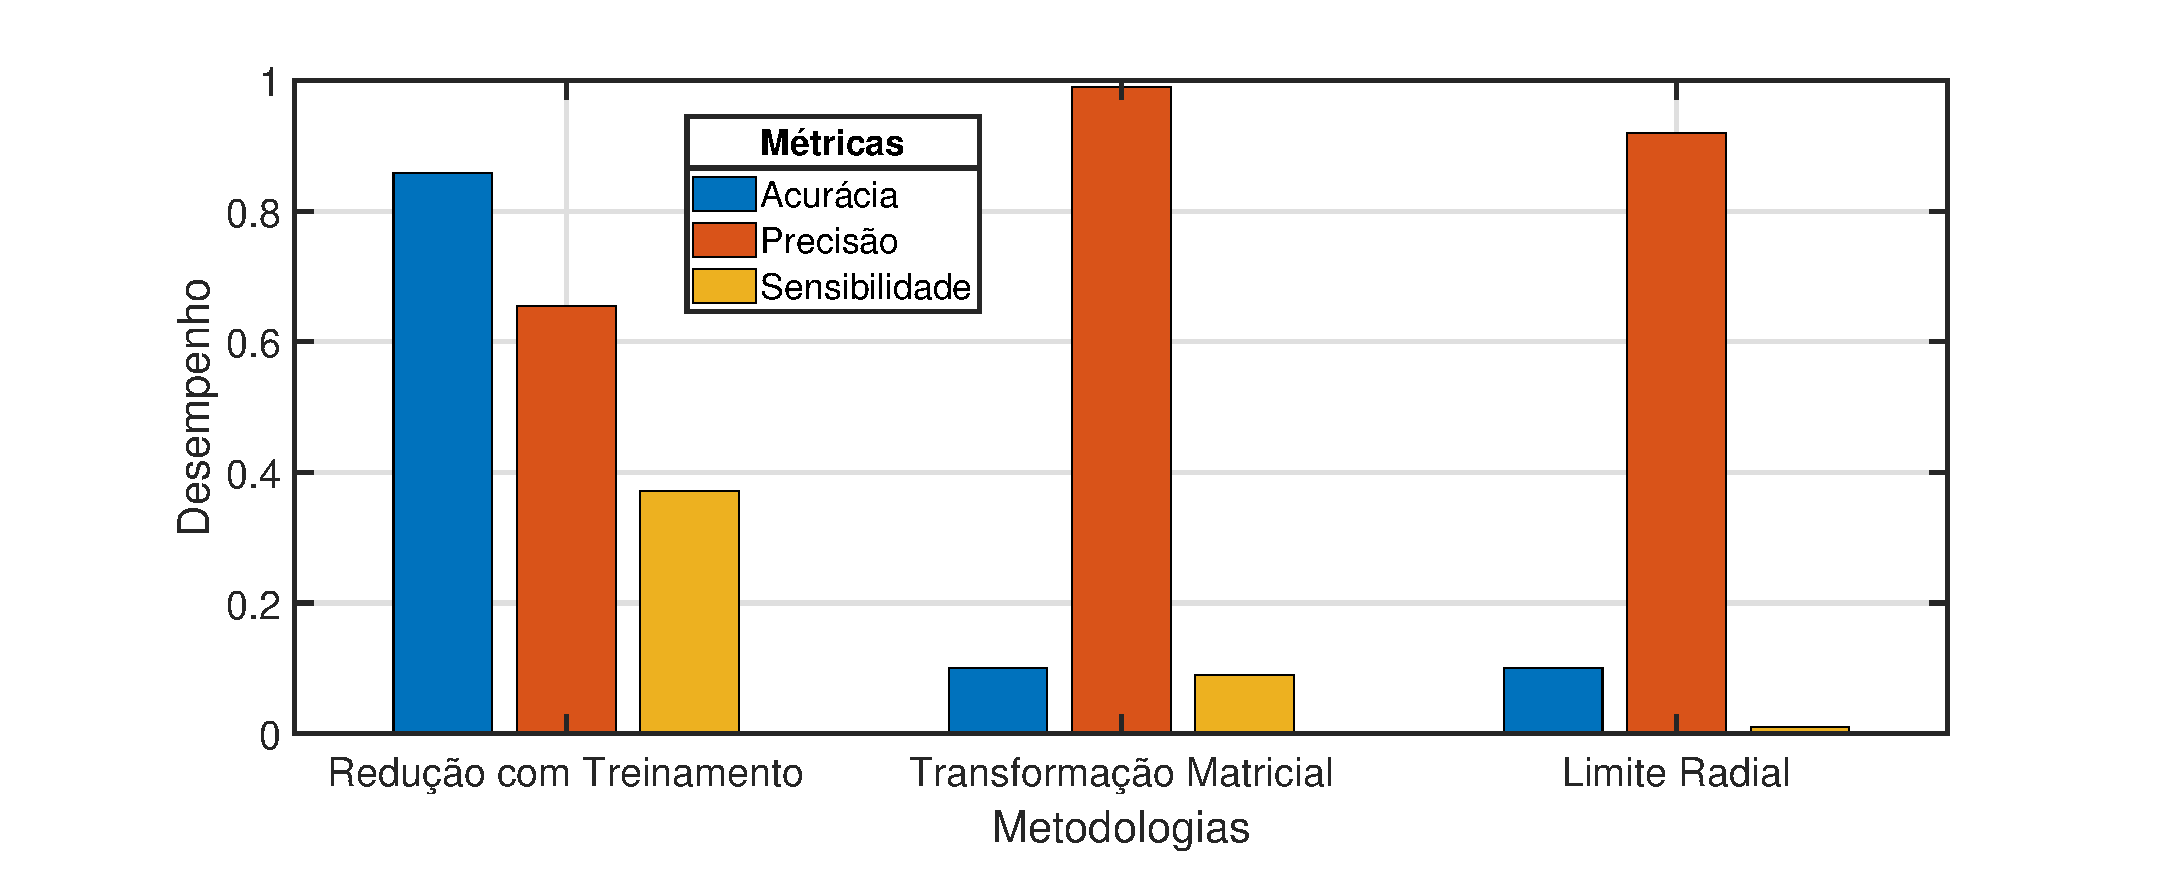
\includegraphics[width=.9\textwidth]{metodologia_fake.eps}
		\caption{Comparação das metodologias revela um comportamento diverso porém ligeiramente complementar nos níveis de recuperação de informação.}
		\label{fig:metodologias}
\end{figure}


\begin{figure}[b!]
	\centering
		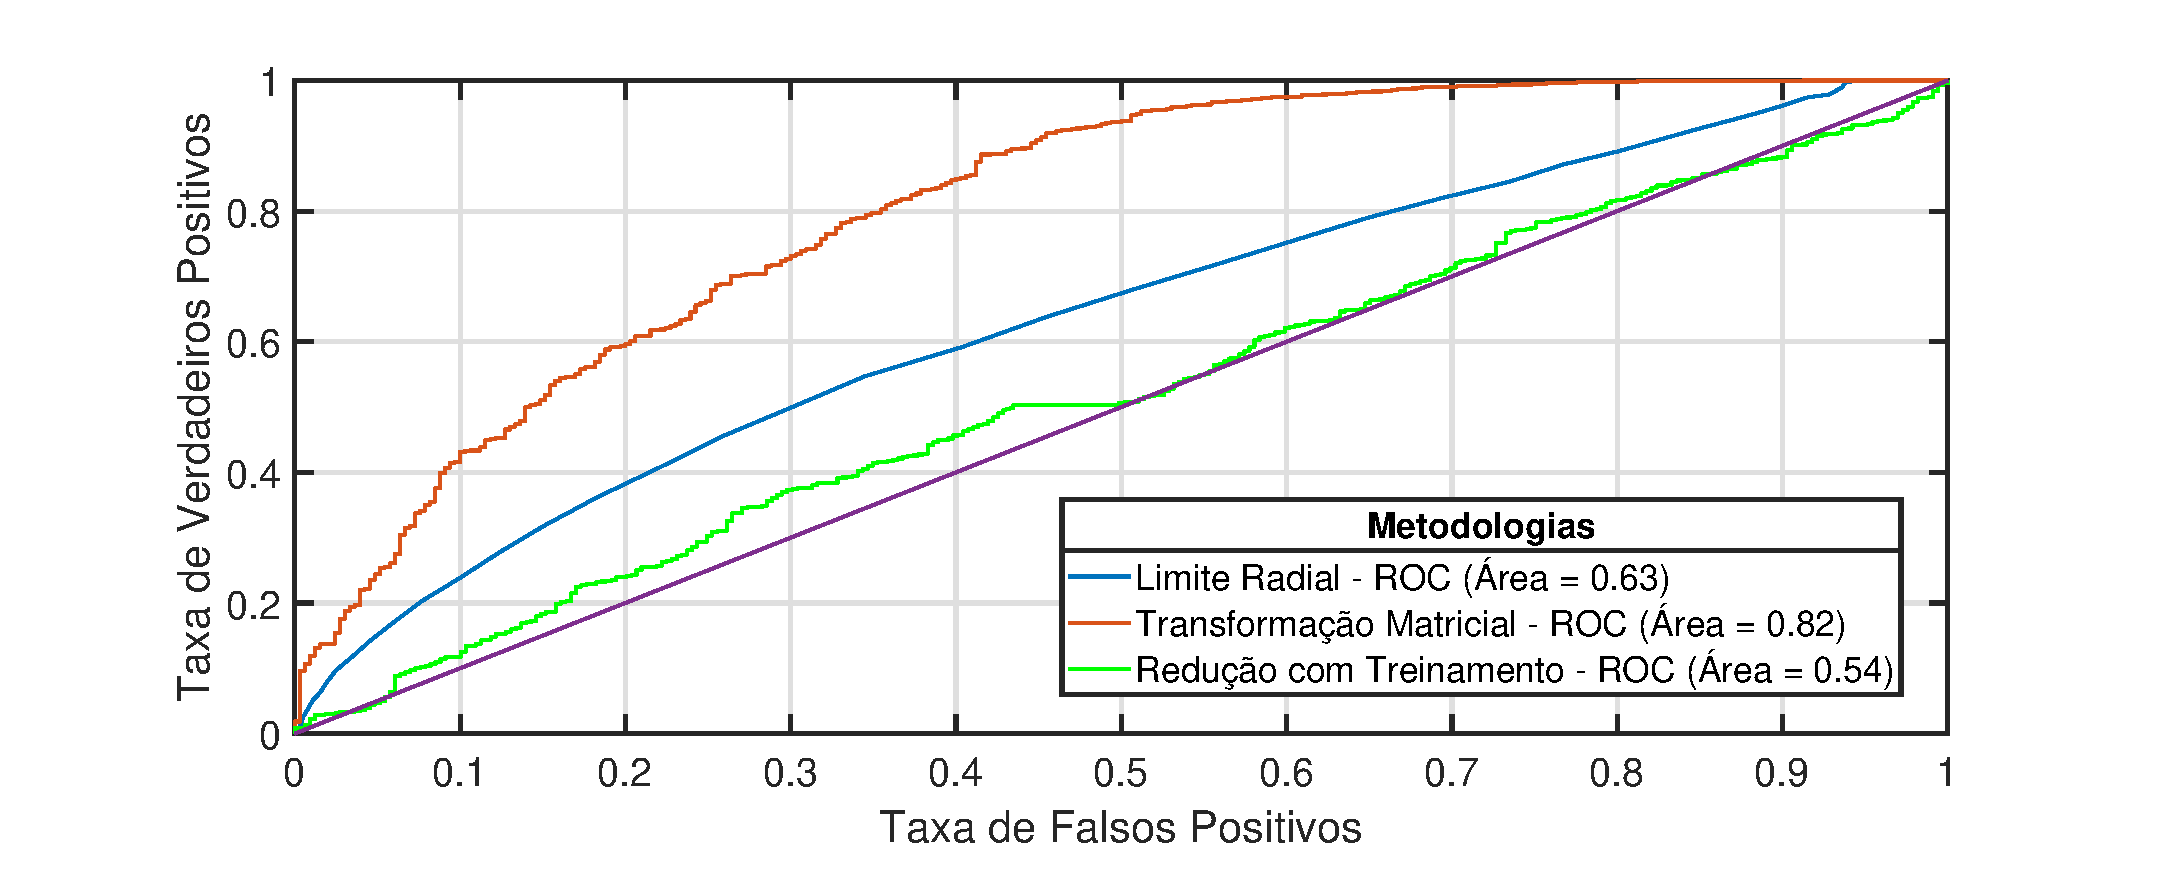
\includegraphics[width=.9\textwidth]{rocs.eps}
		\caption{As curvas ROC refletem o desempenho de um sistema classificador binário à medida que o seu limiar de discriminação varia. Dentre as metodologias, a transformação matricial apresenta o melhor desempenho, visto que possui a maior área acima da reta.}
		\label{fig:rocs}
\end{figure}

Os resultados da primeira metodologia, Redução com Treinamento, demonstram um desempenho mais homogêneo entre as métricas, destacando-se principalmente pela alta acurácia e porcentagem de sensibilidade mais expressiva dentre as três metodologias. Já nos resultados referentes à segunda metodologia, Transformação Matricial, percebe-se uma clara predominância na habilidade de classificar qualitativamente notícias como sendo falsas, expressa pela alta precisão. Em contrapartida, detém baixas porcentagens de acurácia e sensibilidade, essas possivelmente fruto de perdas de características, importantes na diferenciação das notícias, impostas por dois níveis de redução dimensional -- LSI e \textit{k-means}. Analogamente à anterior, a terceira metodologia, Limite Radial, apresenta o mesmo caráter preciso na identificação de notícias falsas embora constate-se uma depreciação nos seus níveis de sensibilidade.


A Figura~\ref{fig:rocs} apresenta uma comparação entre as curvas ROC de cada metodologia de detecção. O bom resultado obtido pela metodologia de transformação matricial, área abaixo da curva de 0,82, baseia-se no fato de que ao realizar o agrupamento com o \textit{k-means}, a dimensionalidade dos dados é substancialmente reduzida, permitindo que a SVM de classe única defina uma hiper-superfície mais ajustada aos dados.

\section{Considerações Finais}
\label{sec:conclusao}

Nesse minicurso foram apresentadas as definições, características e o processo de disseminação de notícias falsas. Em seguida, foram discutidos os métodos tradicionais para a detecção de notícias falsas. Foram comparados os conjuntos de dados de referência mais recentes. Com base em trabalhos da literatura, foi proposto a utilização do Processamento de Linguagem Natural (PLN) na de detecção de notícias falsas. Foram mostrados como o PLN pode ser usado sobre redes sociais e uma comparação com os diferentes métodos de aprendizado de máquina utilizados.
%Este minicurso tenta fornecer uma visão holística do ecossistema de poluição da informação em termos de taxonomia de conteúdos fraudulentos, ciclo de vida de um ecossistema completo, diferentes plataformas de comunicação social digital, principais forças motrizes por trás da disseminação da desinformação e diferentes plataformas de análise de credibilidade. 
Além disso, questões em aberto e desafios também são destacados para explorar as oportunidades de pesquisa em potencial. Esse trabalho é útil para os pesquisadores compreendam os diferentes componentes da comunicação digital \textit{online} de uma perspectiva social e técnica. Divulgação de notícias falsas em várias plataformas multilíngues, estrutura de rede complexa e dinâmica, grandes volumes de dados em tempo real não rotulados e detecção precoce de boatos são alguns problemas desafiadores que ainda não foram resolvidos e necessitam mais pesquisas. 
Finalmente, a atividade prática desenvolvida mostrar a viabilidade na detecção de notícias falsas.
Melhorar a confiabilidade e o futuro do ecossistema de informações \textit{online} é uma responsabilidade conjunta da comunidade científica, formuladores de políticas digitais, administração e da sociedade em geral.




%future work --> https://acm.proxy.uff.br/doi/pdf/10.1145/3305260
%challenges --> https://acm.proxy.uff.br/doi/pdf/10.1145/3305260 2.5

%open issues and future research https://dl.acm.org/doi/pdf/10.1145/3137597.3137600


\bibliographystyle{apalike_br}
\bibliography{main}
\end{document}
